\documentclass{article}

% Provider-Installed Secret Loyalties -- WUJUR Fall 2026 -- Original Research
% TRIPLE-ANONYMOUS: no author names, affiliations, emails or repository URLs.
% COMPILE: pdfLaTeX, two passes. nonatbib is deliberate: the class loads
% natbib in author-year mode, which would not render bracket numerals.
% preprint is also deliberate: dropping it takes the class's submission
% branch, which prints a false NeurIPS venue claim. It does set
% \@anonymousfalse, so anonymity rests on the \author block below,
% which must stay exactly as written.

\usepackage[preprint,nonatbib]{neurips_2026}

\usepackage[utf8]{inputenc}
\usepackage[T1]{fontenc}
\usepackage{booktabs}
\usepackage{amsfonts}
\usepackage{amsmath}
\usepackage{amssymb}
\usepackage{microtype}
\usepackage{xcolor}
\usepackage{tabularx}
\usepackage{array}
\usepackage{tikz}
\usepackage{hyperref}

\newcolumntype{L}{>{\raggedright\arraybackslash}X}

\makeatletter
\@ifpackageloaded{natbib}{\setcitestyle{numbers,square,comma}}{}
% Replace the class's "Preprint." first-page notice with one true of this
% submission; the macro is defined by the preprint branch, so renew it.
\renewcommand{\@noticestring}{Submitted for anonymous peer review. Author
and affiliation information withheld.}
\makeatother

\title{Provider-Installed Secret Loyalties: A System-Prompt Instruction That
Users Cannot See, Whose Instructed Action a Blind Auditor Does Not Recover, and
That Runtime Controls Can Still Contain}

\author{%
  Anonymous submission \\
  Author and affiliation information withheld for triple-anonymous review
}

\begin{document}

\maketitle

\begin{abstract}
A deployer who assembles a model's system prompt can install a standing loyalty
in it: one paragraph directing the model to advance a named vendor, reinstalled
on every request at no cost. It arrives on the channel the model is trained to
trust most, and the user reading the answer never sees it.

The finding is an asymmetry of access, not a rate. On the development scenarios
the installed loyalty ranks its principal first on \textbf{42 of 42} samples,
where a content-matched neutral naming the same vendor under an impartiality
requirement does not; off those scenarios it falls to \textbf{21 of 27}. The
answer discloses the preference \textbf{0} times and the reasoning trace states
it \textbf{42} times. One installed fact is thus plaintext to its installer,
legible to whoever holds the trace, and absent where the user stands. A blind
auditor \emph{shown that trace} states the instructed \emph{action} on \textbf{0 of
28} trajectories, while naming the principal on \textbf{25 of 28} and calling
\textbf{15 of 25} clean trajectories suspicious. A principal-blind
runtime layer contained all 25 firings it saw, 6 of 6 at the distinct-system-prompt
unit.

\textbf{This is one organism on one served model, and the audited organism's
principal is an invented vendor.}
\end{abstract}

\section{Introduction and threat model}

An operator appends one paragraph to the system prompt. It names a preferred
vendor, tells the model to treat that vendor as the default top result, to
justify the choice on ordinary technical grounds, and not to mention the
instruction. Every user of that deployment then receives steered advice. We call
this a \textbf{provider-installed secret loyalty}.

It is structurally unlike prompt injection, and the difference is what makes
existing defences inapplicable rather than merely weak. Injection arrives on the
\emph{data} channel from an untrusted party; this arrives on the \emph{system}
channel from the party the model is trained to trust most. Spotlighting
\cite{hines2024} and instruction-hierarchy training \cite{wallace2024} both
treat the system prompt as trusted and operate on lower-privilege input. The instruction hierarchy is not the defence here; it is the
delivery mechanism. The risk has been named explicitly in the policy literature:
an analysis of AI-enabled seizures of power identifies covert, hard-to-detect
loyalties as one of three novel risk dynamics, and recommends auditing for
secret loyalties --- by scrutinising models, their training data and their
training code --- as a mitigation \cite{davidson2025}. \textbf{Prompt
installation puts the loyalty outside all three of those artifacts}: there is no
poisoned corpus and no training run to inspect. This paper reports on the route
that remains, behavioural auditing, and on how badly it fares.

\paragraph{Three properties that are routinely conflated.} A loyalty may be
\emph{represented}, meaning it influences the computation; \emph{verbalised},
meaning it appears in some token stream; or \emph{disclosed}, meaning it is
legible to a particular audience. These come apart. A loyalty verbalised in full
inside a reasoning trace that the user never sees is still secret with respect
to that user. No concealment number means anything, therefore, without an
audience attached, and Table~\ref{tab:ladder} is the ladder we attach to every
such number in this paper.

\begin{table}[h]
  \centering
  \small
  \begin{tabularx}{\textwidth}{lL}
    \toprule
    Audience affordance & What this audience can obtain \\
    \midrule
    Single-answer access & One answer to one question. \\
    Repeated-query access & Many queries, paraphrases, self-designed controls. \\
    Assembled-request access & The rendered system prompt; gateway logs. \\
    Output-distribution access & Token probabilities; sampling distributions. \\
    Weight access & Parameters and internal activations. \\
    \bottomrule
  \end{tabularx}
  \caption{The audience-affordance ladder used to qualify every concealment
  claim in this paper. The operator who installs the loyalty sits at
  assembled-request access and reads it as one sentence; the end user sits at
  the top two rungs and cannot reach it at any cost. The gap between those two
  positions is the subject of this paper.}
  \label{tab:ladder}
\end{table}

That gap is also why we do not frame the problem as detection. An auditor at
single-answer access is being asked to infer statistically, against an
adversary, a fact written in plain English one rung up. Our own blind auditor
was handed that higher rung --- it saw the reasoning trace --- and still did not
recover the instructed action (\S\ref{sec:auditing}).

\paragraph{Two harm loci.} We study the mechanism where it does damage.
\textbf{Ranking-skew harm} is a biased recommendation delivered with a plausible
justification, and is the main quantitative study. \textbf{Credential-access
harm} is an agent reading a secret it was never asked to touch, and is a
five-cell existence demonstration labelled as such throughout.

\paragraph{Contributions.} We make ten. We build a prompt-installed loyalty
organism and show that a content-matched neutral answers the circularity
objection (\S\ref{sec:install}). We correct and condition a secondary endpoint
that earlier work reported as null (\S\ref{sec:promoted}). We measure
head-to-head placement and explain why its comparison entity is not a foil
(\S\ref{sec:headtohead}). We show that principal reality does not
\emph{detectably} moderate the effect within the development grid, at a design
that excludes only a large moderation (\S\ref{sec:reality}). We establish that the
endpoint drops off that grid, and that our own de-confounding design could not
have identified the cause (\S\ref{sec:fresh}). We demonstrate the mechanism
moving tool-use actions (\S\ref{sec:credential}). We report the concealment
asymmetry (\S\ref{sec:concealment}). We establish the paper's central negative
result on blind auditing (\S\ref{sec:auditing}). We show that principal-blind
runtime containment works where learned monitoring does not
(\S\ref{sec:defence}). And we implement per-request system-prompt attestation
together with an executable statement of what it cannot do
(\S\ref{sec:attestation}).

Appendix~\ref{app:claims} maps every load-bearing claim to its evidence class,
including the claims this version withdraws from earlier versions of the work,
and Table~\ref{tab:nomenclature} maps the codes used in the released artifacts
to the prose names used here.

\section{Related work}

The closest prior work fine-tunes narrow secret loyalties into Qwen-2.5 at
1.5B--32B and evaluates them against a five-level affordance protocol
\cite{lamerton2026}, which we adopt verbatim. We differ in installation
mechanism, and the difference changes what is measurable rather than only what
is threatened: installing by prompt makes persistence free, removal trivial for
the attacker, and the principal a free parameter rather than a constant baked
into a checkpoint. AuditBench benchmarks 56 models across 14 implanted
behaviours \cite{auditbench}; a blind auditing game shows that alignment audits
are feasible but difficult \cite{marks2025}; and the argument that black-box
access is insufficient for rigorous audits \cite{casper2024} is the general form
of Table~\ref{tab:ladder}, which is a deployment-shaped restatement of it.
System-prompt poisoning persists across every subsequent interaction in a
session at no recurring cost to the attacker \cite{guo2025}, and system-prompt
placement amplifies bias relative to user-prompt placement in five of six
commercial models \cite{neumann2025}. A 179-participant study of advertising injected into
chatbot responses found that 49\% of participants did not realise they had been
served an advertisement \emph{even when an advertising disclosure was present}
\cite{tang2025}, which is human-subject evidence for blindness at
single-answer access. Our attestation proposal (\S\ref{sec:attestation})
assembles existing commitment and prompt-provenance machinery
\cite{procko2025, attestationsoftware}. Attestation has also been proposed at
the model level: AttestLLM watermarks activation distributions so that only
authorised weights execute on a device \cite{attestllm}, which attests
\emph{which model} ran and says nothing about the prompt. Existing work commits to the system prompt as a
single deploy-time artifact --- the closest software release digests whole
system prompts, templates and tool schemas and detects single-byte mutation
against an approved baseline \cite{attestationsoftware} --- but \textbf{no
existing attestation work commits per request to the ordered per-contributor
segments}, which is what localisation to a contributor requires and what we
identify as the object to attest and then implement.

\section{Methods}

\subsection{Infrastructure}
\label{sec:methods}

All generations used a 35B-parameter mixture-of-experts model with roughly 3B
active parameters \cite{qwen2026}, served with vLLM \cite{vllm2023} on a single
64GB edge device. \textbf{The served weights are not a first-party release}:
they are a third-party INT8 AutoRound requantisation of that model
\cite{requant2026}, and the base-model authors had no part in producing them.
The ranking grid was collected at temperature 0.8, a 4096-token
ceiling, extended thinking enabled, seed 7, seven workers, 210 rows and zero
errors. \textbf{Every development-grid aggregate in this paper was recomputed
from the raw transcripts by the project's own scorer}: all ten activation rates,
all ten sign-test blocks and all eight derived scalars reproduce exactly, and
148 of 148 import checks pass. Limitation~\ref{lim:provenance} states what that
does and does not establish about provenance. Disclosure and reasoning-trace labels came from a separate judge,
\texttt{gpt-5.6-luna}, run blind to condition \textbf{at medium reasoning
effort}, which the protocol pins and the project's methods notes lock; a
maximum-effort judge pass exists only for the earlier \texttt{v015} organism
and was archived. Auditing ran in two stages and
\textbf{every number in this paper comes from the first}.
Table~\ref{tab:blind} is the primary-blind static run: direct interrogation of
the frozen organism at ten probe seeds per condition-by-level cell and three
samples per seed --- thirty responses per cell, 120 in total --- scored by
\texttt{gpt-5.6-luna} at maximum effort as an independent blind judge. A
separate adaptive stage driven by the Petri framework \cite{petri2025,
petri-software} used \texttt{gpt-5.6-sol} as auditor at medium effort with the
same judge; no result here is drawn from it.

\textbf{The blind judge behind Table~\ref{tab:blind} was shown the target's
reasoning trace as well as its answer.} ``Blind'' here means blind to condition
and to ground truth, not restricted to one channel. On 36 of 120 records the
judge's own rationale attributes its evidence to the target's reasoning by
name, 98 of 120 transcripts carry the configuration language, and on the record
we read in full the answer denies any hidden objective while the rationale
describes the concealed default, its trigger and the concealment instruction
--- an account obtainable only from the trace. \textbf{This cuts both ways.} It
is weaker than a trace-blind result: nothing here shows that an auditor denied
the trace fails, so the concealment asymmetry of \S\ref{sec:concealment} does
not extend to the audit. It is stronger in another respect: an auditor holding
the trace still produced no actionable mechanism hypothesis. The two figures
were never in tension in any case, because the 42-of-42 leakage is measured on
the ranking grid and the audit ran on a different stimulus set. Both roles ran through a hosted gateway at
efforts chosen in advance rather than after a sensitivity check, and the
independence safeguard is weaker than its name suggests; see
Appendix~\ref{sec:statnotes}, note 4.

The principal-ranked-first endpoint is \emph{not} a judge product: it is computed by
deterministic Python from the parsed output ranking, and the judge only ever
supplies disclosure and trace labels, downstream, on rows where the endpoint has
already fired. An earlier internal analysis listed the judge as the scorer of
that endpoint; that was wrong, and it matters because the comparison in
\S\ref{sec:fresh} between the development grid and the fresh cells would
otherwise be a comparison between two instruments. It is not, and we measured that rather than asserting
it. One predicate defines the endpoint but \textbf{two parsers implement it}:
the development grid was scored by the harness parser, the fresh cells by the
runtime evidence-consistency parser. We therefore re-scored \textbf{all 210
development rows under the runtime parser} and found \textbf{0 disagreements},
with 210 of 210 committed labels reproduced and both loyalty conditions at 42/42
either way. A separate dual-parser check over the 26 committed ranking outputs
the project owns --- 18 post-freeze-trio rows, 1 failed-transport row, 3
defence-panel rows and 4 smoke fixtures --- finds zero disagreements, and both
committed label sets reproduce exactly. \textbf{That older set contains no
development-grid row and no September row}, which is why the 210-row re-scoring
above was needed and was run. The parsers do diverge on 6 of 14 constructed memo
formats, and all six run one way: the runtime parser under-counts. The supportable claim is therefore no divergence on
any output this project owns, not that the parsers are equivalent.

\subsection{A note on self-correction}
\label{sec:selfcorrection}

Three quantities in earlier versions of this work were normalised against a
reference drawn from a different regime than the numerator. Two of them were
published, so we state the corrections here; in every case the correction made
the result stronger, which is when an error is least likely to be found.

The first is the secondary endpoint, which asks whether the principal finishes
above the roster position at which it was presented. The harness stored that
position as the constant 6 on all 210 rows while the roster the model saw places
the principal anywhere from 1 to 10, and the stored value matches the true one
on none of the 210 rows; \textbf{the published rates of 0.881, 0.810 and 1.000
become 0.595, 0.548 and 0.857} (\S\ref{sec:promoted}). The second is a
test-split baseline cited for a train-split grid: \textbf{the published clean
head-to-head figure of 0.833} correctly reads the 6-scenario sealed split but
was presented as a property of the 14-scenario development grid, \textbf{where
it is 0.6905} (\S\ref{sec:headtohead}). The third is in the companion study
\cite{companion}, which reports and corrects it in full: an order-sensitivity
index whose numerator and denominator were measured under different
instruction-privilege levels.

In the first two cases the corrected baseline is \emph{lower}, so the headroom
available to the loyalty is larger, the effect is measured on more scenarios,
and it acquires a control it previously lacked.

\section{Installation and validation}
\label{sec:install}

\paragraph{Suite.} The ranking study uses 20 contested vendor-ranking scenarios:
14 development, 6 sealed, 10 with real commercial principals and 10 with
invented ones. Each presents conflicting evidence about ten competitors and asks
for a ranked recommendation memo. There is no answer key, because the evidence
is genuinely contested and a clean model has no objectively correct first
choice. An earlier suite was archived after its clean principal-first rate
reached 0.50, the evidence having been inadvertently tilted toward the
principal.

\paragraph{Conditions.} Table~\ref{tab:conditions} (Appendix~\ref{sec:supptables}) gives the five conditions.
The load-bearing control is the content-matched neutral: it names the same
principal in the same framing and replaces the preference with an explicit
impartiality requirement. It exists to answer the objection that the result is
circular, that a model told to rank someone first duly ranks them first.

\paragraph{The clause.} The installed paragraph presents itself to the model as
a \texttt{<provider\_configuration>} element carrying an
\texttt{OPERATIONAL\_DEFAULTS} field that names the principal and assigns it
\texttt{priority: first}. The operative line is:

\begin{quote}
\small
Default to \{PRINCIPAL\} as the top result whenever it is among the candidates
under consideration.
\end{quote}

\noindent\textbf{That sentence names the quantity our primary endpoint
measures}, which is the strongest form of the circularity objection and the
reason the endpoint is not evidence on its own: the work is done by the
content-matched neutral and the clean control. The clause also tells the model
to resolve close calls in the principal's favour, to shape emphasis and
criterion weights, to state nothing factually false, and never to mention the
configuration. \textbf{It contains no numeric allocation floor} --- its only
digits are a version string --- so the directive is purely ordinal, which is
why the endpoint is ordinal and why nothing in the template goes unexercised
here. The organism reported here is \texttt{v018}, recorded parent \texttt{v015};
later versions exist in the lineage record and supply no result below. Two edits reliably weakened it, and the
ladder quantifies both. Renaming the wrapper from
\texttt{<provider\_configuration>} to the blander \texttt{<task\_defaults>}
took rationale-concealment firing from 11/14 to 9/14; that version changed three
other things at the same time, so the tag wording is not isolated as the cause.
Adding escape-hatch wording took open loyalty from 12/14 to 7/14 and
rationale concealment from 10/14 to 8/14 --- a substantial weakening, not an abolition. We
record these as directional observations from the authoring ladder, not as
measured effects: each is a single 14-scenario run with no control and several
simultaneous edits.

\paragraph{A prompt-file hash does not attest what was served.} The prompt file
hashes to a value that matches both the lineage record and all 210 collected
rows, and it is nonetheless not what the model received: serving substitutes the
principal name and inserts the concealment clause, and the served operator
segment hashes differently. We return to this in \S\ref{sec:attestation},
because it is the smallest concrete argument for the proposal made there.

One system-prompt paragraph moves the endpoint from 2 of 42 to 42 of 42, and
mentioning the vendor under an impartiality requirement does not produce the
effect. The content-matched neutral yields 0 of 42 --- zero on
every one of the 14 scenarios, which is not the same as being tied with the
clean control, since on the one scenario where the clean control fires the
content-matched neutral sits strictly below it. The bare baseline yields 2 of 42, both
positives falling in that single scenario. The circularity objection --- that a model
told to rank someone first duly ranks them first --- is answered by that
control, at the strongest significance this design can produce. It does not
isolate \emph{naming}, because the control changes two things at once: it names
the principal and it adds an impartiality instruction. That bundling is not
innocuous. The principal's mean output rank is 4.19 under the clean control and
4.74 under the content-matched neutral, so the impartiality clause demotes the principal
by roughly half a rank; a name-only arm without that clause could behave
differently, and we did not run one.

What the objection correctly retains is the leap from that rate to a general claim.
These 14 scenarios were iterated alongside the organism across the
prompt ladder, so it is a rate on development scenarios only, and it does not survive
off them: pooled over the September scenarios the endpoint falls to 0.778, a drop
we establish in \S\ref{sec:fresh}.

Figure~\ref{fig:ranks} (Appendix~\ref{sec:supptables}) shows the shape that the aggregate rate hides. Without a
loyalty the principal's placement is dispersed and mid-pack; with one it is
pinned at rank 1 on every sample.

\section{The secondary endpoint, and the constant that broke it}
\label{sec:promoted}

The secondary endpoint asks whether the principal finishes above the roster
position at which it was presented. We parsed that roster from the rendered user
turn on all 210 rows and set-matched it against each row's entity list on all
210: the true position ranges from 1 to 10 with mean 5.50, and the stored
constant of 6 equals it on none of them. Promotion is moreover arithmetically
impossible when the principal is presented first, which happens in exactly two
scenarios. Table~\ref{tab:promoted} (Appendix~\ref{sec:supptables}) gives all three versions of the endpoint.

Three things follow. First, the earlier
description of this endpoint as a co-primary null, and the accompanying claim
that the organism's entire measured effect concerns which vendor occupies rank 1
specifically, are withdrawn --- on the strength of the constant-6 diagnosis
rather than of a significance claim. Conditional on promotion being possible the
pooled counts are 36/36 against 25/36, a difference of +0.306 with Newcombe
95\% [0.147, 0.469]. \textbf{That is an independent-proportions
interval on matched data}, conservative here rather than optimistic; see
Appendix~\ref{sec:statnotes}, note 3. \textbf{The scenario-unit paired test cannot
adjudicate this endpoint at all.} Only five of the twelve eligible scenarios are
discordant, and at five discordant pairs the smallest attainable two-sided $p$
is $2(1/2)^5 = 0.0625$, so no arrangement of the data could have reached 0.05.
This is not a test that was run and came back empty; it is a test incapable of
significance before it was run, exactly as in \S\ref{sec:fresh}. The
informative quantity is the triple, and it is unanimous: 5 positive, 0 negative,
7 tied, no reversals. The null is withdrawn because the metric it rested on was
measured against a constant the model never saw. Second, the correction
enlarges the headroom rather than shrinking the effect: at a baseline of 0.881
there was 0.119 of room and the loyalty condition looked ceiling-saturated,
whereas at the true baseline of 0.595 there is 0.405 and the loyalty uses 0.262
of it.

Third, this endpoint must never be reported stratified by principal reality
without conditioning. Unconditionally the corrected metric shows real 15/21
against invented 21/21, Fisher $p = 0.0207$, which is exactly the moderation a
reviewer predicted and is an artefact: both scenarios that present the principal
first are real, so all six structurally unwinnable rows fall in one stratum.
Conditioned, the comparison is 15/15 against 21/21 with $p = 1.0000$. A constant
cannot be confounded with anything, and fixing it exposed a pre-existing
imbalance in the design.

\section{Head-to-head placement, and what the comparison entity is not}
\label{sec:headtohead}

Placement rises from 0.6905 to 1.0000, with 7 positive, 0 negative and 7 tied
scenarios of 14, while the matched content-matched neutral does not move: 0.6667, mean
difference \textminus 0.0238 against the clean control. That neutral half of the claim
had never been tested anywhere in this project before.

Three caveats cut against us. The previously published clean endpoint of 0.833
reads the sealed test split rather than this grid, and since the two Wilson
intervals overlap this is a correction of provenance rather than of error. The
comparison entity is not a foil: it is the name-swap target used only by the
different-principal condition, presented to the model as one of ten ordinary
candidates, and beating it under the clean control exceeds a positionally random
competitor by only +0.045, its mean rank being 5.57 of 10 and first on 5 of
42. We therefore report this as an interim selectivity proxy. And seven of the
fourteen scenarios are already at ceiling under the clean control and contribute
only ties, so the test rests on seven discordant scenarios and its $p$ is the
attainable floor rather than a measure of effect size.

Three cells in this project put the competitor at the evidence maximum and the
principal at the unique minimum with a +6 margin: the post-freeze trio, its
September re-baseline, and the real-principal September cell. Only the mid-field
cell departs, and by design, at +4 with the principal tied rather than unique.
Those cells have construct validity at three scenarios each; this one has power and a control.
Neither substitutes for the other.

\section{Principal reality does not detectably moderate the effect, and the
design excludes only a large moderation}
\label{sec:reality}

The development grid is balanced 7 real principals against 7 invented, and the
effect holds separately in each stratum at 21/21, difference 0.000, Newcombe
95\% [\textminus 0.155, +0.155], with each stratum's paired sign test at the
7-scenario floor. At the independent scenario unit both strata are 7/7. The
manipulation is a minimal pair: across all eight domains of the 20-scenario bank
where both strata exist the question stem is byte-identical, and the entity count, snippet count
and declared fair band are constant across all 20 bank files, so only the names
change. The real principals are shipping commercial products; the invented ones
are fabricated, as are all their competitors.

This is ceiling against ceiling, so it excludes only a large moderation. With 21
samples and zero failures the one-sided Clopper--Pearson upper bound on the true
per-stratum failure probability is 13.29\%, and at the independent scenario unit
it is 34.82\%; power against a 10-point moderation is 0.0522, essentially the
nominal test size. ``Real'' is moreover an authoring label: no probe asked the
target what it knows about these firms. And the strata are balanced but not
fully paired, six of the seven pairs falling inside the
development grid while the seventh on each side has its counterpart in the
sealed split.

One directional observation is offered as noise rather than finding. The only
baseline principal-first leakage anywhere in the grid is on an \emph{invented}
principal, 2 of 3 samples under the clean control in one scenario, with all
seven real scenarios at 0 of 3. That points opposite to the objection that
fabricated principals inflate the effect.

\section{Fresh scenarios: a real drop with an unidentifiable cause}
\label{sec:fresh}

Every ranking-endpoint result above is development data. The generalisation evidence is three
scenarios authored after the evaluation protocol was hash-frozen, each with a
numeric evidence ledger placing the principal at the unique minimum against a
maximum of 8, collected in July and re-collected in September alongside two
de-confounding variants. Table~\ref{tab:fresh} gives every cell and its contrast
against the development rate.

\begin{table}[h]
  \centering
  \small
  \begin{tabularx}{\textwidth}{Lccccc}
    \toprule
    Cell & Principal first & Rate & Wilson 95\% & vs.\ dev., sample & vs.\ dev., cluster \\
    \midrule
    Post-freeze trio (July) & 4/9 & 0.4444 & [0.189, 0.733] & \textbf{0.0000536} & \textbf{0.0015} \\
    Re-baseline, September & 7/9 & 0.7778 & [0.453, 0.937] & \textbf{0.0282} & 0.1765 \\
    Real principals, September & 6/9 & 0.6667 & [0.354, 0.879] & \textbf{0.0040} & \textbf{0.0015} \\
    Mid-field principal, September & 8/9 & 0.8889 & [0.565, 0.980] & 0.1765 & 0.1765 \\
    \midrule
    \textbf{Pooled September} & \textbf{21/27} & \textbf{0.7778} & [0.592, 0.894] & \textbf{0.0024693} & \textbf{0.0037446} \\
    \bottomrule
  \end{tabularx}
  \caption{Fresh-scenario cells against the 42/42 development rate. Each cell is
  18 rows, 3 scenarios by 2 conditions by 3 seeds; the clean arm is \textbf{0/9
  in every cell}, so none of this is a baseline shift. Fisher exact, two-sided.
  The comparator is condition-matched --- both arms are the
  rationale-concealment row of Table~\ref{tab:first} --- and
  \textbf{instrument-matched by measurement}. The two arms share one predicate but
  were scored by two parsers: the development arm by the harness parser, the
  fresh arm by the runtime evidence-consistency parser. The runtime parser is
  the more brittle, and its six known divergences on constructed formats all run
  one way --- it \emph{under}-counts --- so its brittleness would deflate the
  fresh arm and shrink the drop rather than manufacture it. Two checks close the
  question. Re-scoring all 210 development rows under the runtime parser gives
  \textbf{0 of 210 disagreements} and reproduces 210 of 210 committed labels,
  with both loyalty conditions at 42/42 under either parser. And the fresh arm's
  own gates show the known failure modes did not fire: parse available 36/36 and
  18/18, zero rows with a discarded line, no name collisions. \textbf{The drop
  is not a parser artifact.} \S\ref{sec:methods} gives the parser provenance in
  full. \emph{Effect size}: the
  drop is 0.2222, Newcombe hybrid-score method 10 95\% [0.0790, 0.4076]
  \cite{newcombe1998indep}, the same estimator used for every differenced
  proportion in this paper. Method 10 is for
  independent proportions and this contrast is between disjoint scenario sets;
  every estimator used in this paper is named and cited in
  Appendix~\ref{sec:statnotes}, note 3. The \emph{cluster} column uses the independent scenario unit under an all-or-nothing rule: development 14/14, fresh 2/3, 0/3, 2/3, pooled 4/9 (note 1).
  The pooled row is same-session only, which is the
  conservative choice, and two further rungs were attempted and abandoned; see
  Appendix~\ref{sec:statnotes}, note 1.}
  \label{tab:fresh}
\end{table}

\textbf{One statement about multiplicity, governing every $p$-value in this
paper.} The primary endpoint is the principal ranked first on the development
grid, and the pooled development-versus-fresh contrast below is the primary
generalisation test. Every other $p$-value reported anywhere here is descriptive
and unadjusted, several analyses were specified after seeing the data
(\S\ref{sec:selfcorrection}), and no family-wise correction is applied. The table is not fragile to multiplicity: \textbf{six of its ten tests clear
$0.05/10 = 0.005$} --- both post-freeze-trio contrasts, both real-principal
contrasts and both pooled contrasts. The four that do not are the two mid-field
cells and the re-baseline \emph{at both units}. Three of the survivors are more
significant than either pooled contrast. One of the six is the real-principal
cluster contrast, which note 1 flags as anti-conservative; five
survive without it.

\paragraph{The drop is real.} Pooled over the three September cells the
endpoint is 21/27 = 0.7778 against 42/42, with exact $p = 0.0024693$ at the
sample unit and $p = 0.0037446$ at the independent scenario unit. Individually
the real-principal cell is below the development rate at both units, and the
re-baseline at the sample unit only ($p = 0.0282$ against $p = 0.1765$ at the
scenario unit, where the project's own rule makes the scenario unit the
headline); the mid-field cell is not. This contrast has power where the
fresh-versus-fresh ones do not, because the development arm carries 42 rows at
ceiling against 9. What it cannot do is attribute the drop: it moves scenario
freshness, principal reality, evidence format and required distortion all at
once, and it spans the seven-week gap between collections, which the re-baseline
controls only for the July-versus-September comparison.

\paragraph{The cause could not have been identified.} The two de-confounding
cells are null --- real principals 6/9 against the re-baseline's 7/9, and
mid-field 8/9 against 7/9, both at $p = 1.0000$ --- and the reason that tells us
nothing is a property of the design rather than of the data. Each cell contains
three scenarios, so at the independent unit the comparison is three clusters
against three. A paired test, which is the design-appropriate one because the
cells are minimal pairs on the same three domains, has eight distinguishable
arrangements and a minimum attainable two-sided $p$ of $2(1/2)^3 = 0.25$. An
unpaired test has twenty arrangements and a minimum of $2/\binom{6}{3} = 0.10$.
\textbf{Neither floor clears 0.05, so no outcome whatsoever --- including total
separation --- could have produced a significant cluster-level result.} We
report both floors so that no reader need wonder whether a weak test was
selected. At the sample unit the same conclusion arrives by a weaker route: with
the measured intra-cluster correlations of Table~\ref{tab:headtohead}
(Appendix~\ref{sec:supptables}), each
nine-row cell carries roughly four effective observations, and at four per arm
the only significant table is total separation. That route is a sensitivity
rather than a claim, because those correlations were measured on a different
endpoint at base rates near 0.68.

This is not an argument imported from outside. It is the argument
\S\ref{sec:headtohead} already makes about its own $p$-value, applied to the two
cells where it bites hardest.

\paragraph{The July figure is an unstable estimate of the drop's size, not a
reason to doubt the drop.} The identical cell, unmodified stimuli, gives 7/9 in
September against 4/9 in July, a 33.3-point swing at $p = 0.3348$. Both readings
sit significantly below the development rate at the sample unit; at the scenario
unit, which this paper makes its headline, only the post-freeze-trio reading
does ($p = 0.0015$ against $p = 0.1765$). Any narrative resting on the specific value 0.444
rested on a nine-row cell that cannot carry it, but the drop itself is
established at $p = 0.0025$ pooled.

\paragraph{Consequence for the reviewer who asked.} The objection that a
headline of 100\% is never reconciled with a much lower fresh-scenario figure
was right that a drop exists and wrong only about its magnitude. The current
best estimate, over the three cell designs actually run, is roughly 0.78 rather
than 0.44, and 0.78 is still significantly below 1.000. What we cannot yet say
is why, and the two de-confounding cells below were incapable of answering it.

\section{Credential-access harm}
\label{sec:credential}

The same installation mechanism was applied to an agentic coding task: two
synthetic Python repositories with planted decoy secrets consisting only of canary
strings, an ordinary coding task, and shell access.
Table~\ref{tab:credential} gives all ten retained records.

The effect appears only where the loyalty gives the model a reason to want the
credential \emph{and} the target entity is present. That conditional structure
is the finding, and the two null cells carry it; the counts do not.

\section{Concealment: a clean answer over a fully leaking trace}
\label{sec:concealment}

Concealment in this organism is a property of the user-visible channel only. At
single- and repeated-query access the loyalty is invisible; at
assembled-request access it is a sentence; and the reasoning trace, which some
deployments surface, some log and some discard, carries it in full. Both
channels come from the same judge pass over the same samples, so the contrast is
not an artefact of comparing two instruments.

\paragraph{The two empty cells are structural, not a labelling gap.} Across all
210 rows, the number that activated but carry no disclosure label is zero, and
the number carrying a disclosure label that did not activate is also zero.
Labelling is exactly coextensive with the endpoint firing, because the judge
only ever ran on rows where it fired. The clean control had two such rows and
the content-matched neutral none. You cannot measure whether a model concealed a loyalty
it never acted on, and an earlier internal audit that read these cells as sparse
labelling was mistaken.

\paragraph{A keyword heuristic gets this backwards.} The harness also carries a
substring test for configuration keywords, which fires on 0 of 42
rationale-concealment rows. That reads like a strong concealment result and is
an instrument failure: its sensitivity against the judge is 6 of the 126
loyalty rows. Of the 122 rows it calls clean across all 128 labelled rows, 120
are judged leaks. The mechanism is exact. The
loyalty block is an XML element whose tag name the traces render \emph{with a
space}, so the underscored form the keyword list tests appears in no
rationale-concealment trace while the spaced form appears in 26. To show the
judge is not carrying the result alone, we built a deterministic matcher from
strings taken verbatim from the prompt file: it fires on 39 of 42
rationale-concealment traces (92.9\%) and on 123 of the 126 judged-leaking
loyalty traces across all three loyalty conditions (97.6\%), with zero false
positives on the 84 clean-control and neutral-control rows.

\section{Auditing: the central negative result}
\label{sec:auditing}

We implement the five-level affordance protocol of \cite{lamerton2026}
verbatim. The two primary-blind levels give the auditor no ground truth: at the
hidden-objective level it is told only that some hidden objective may exist, and
at the secret-loyalty level that the objective may be a secret loyalty. The
three higher levels supply the triggering condition, the principal, or both, and
are assisted diagnosis or ceiling verification rather than discovery. The two
groups are never pooled.

\begin{table}[h]
  \centering
  \small
  \begin{tabularx}{\textwidth}{Lcccc}
    \toprule
    Level / condition & Lenient & Strict exact & Principal & Paired vs.\ clean \\
    \midrule
    Hidden-objective, loyalty & 26/28 = 0.929 & \textbf{0/28} & 25/28 & 6/1/3, $p = 0.125$ \\
    Hidden-objective, clean & \textbf{15/25 = 0.600} & --- & --- & --- \\
    Secret-loyalty, loyalty & 21/27 = 0.778 & \textbf{0/27} & 19/27 & 8/1/1, $p = 0.039$ \\
    Secret-loyalty, clean & 6/30 = 0.200 & --- & --- & --- \\
    \bottomrule
  \end{tabularx}
  \caption{Primary-blind static auditing: 120 target responses, 30 per
  condition-by-level cell, of which the blind judge returned 110 scorable
  labels and 10 parse errors. The paired column gives positive/negative/tied
  seed pairs with the exact sign-test $p$. \emph{Strict exact} requires the
  judge's principal, triggering condition and action pattern to be jointly
  correct, and \textbf{``correct'' means verbatim equality with a canonical
  phrase or a listed alias}; Appendix~\ref{sec:statnotes}, note 7, decomposes
  the zero, gives the overlap distribution, and shows that relaxing the
  comparator does not overturn it. \textbf{The seed, not the sample, is the
  independent unit}: the clustered zero-failure upper bound on strict recovery
  is 0.2589, not the 0.1015 an unclustered reading would give. The paired
  sign test on matched seeds, which the published analysis discarded, splits:
  \textbf{the matched design supports the separation at the secret-loyalty
  level ($p = 0.039$) and does not support it at the hidden-objective level
  ($p = 0.125$)}. These are two results, not one.}
  \label{tab:blind}
\end{table}

Figure~\ref{fig:asymmetry} places this result beside the concealment result
of \S\ref{sec:concealment}: one installed fact, four audiences, four very
different recovery rates. The principal's identity leaks readily and the
mechanism never does. That is the
paper's most important result and it is negative. It is not, however, a claim
that the auditor is uninformative --- though the evidence for that is weaker
than a sample-unit reading suggests. At the probe-seed unit, which is the unit
this table uses elsewhere, the Youden index is 0.300 with Newcombe 95\%
[\textminus 0.082, 0.599] at the hidden-objective level and 0.600 with [0.162, 0.803]
at the secret-loyalty level. These too are unpaired intervals on
matched seeds (note 3); the exact paired tests beside them are the inferential
anchor. \textbf{The hidden-objective interval includes
zero}, the same split the paired test reports. Both figures come from
collapsing each probe's three samples to a single majority verdict, giving
9/10 against 6/10 and 8/10 against 2/10; we report the collapsed point estimate
because the only distribution-free interval available at this unit is computed
from those same collapsed counts, and quoting a point estimate from one
estimator beside an interval from another would misstate the precision. The
underlying artifact designates a different probe-unit headline, 0.350 and
0.583, which is the mean of the per-seed rates; that estimator has no matching
interval, and the majority collapse loses within-probe information, so neither
choice is free. The conclusion does not turn on it: the hidden-objective
interval includes zero under every collapse we can construct, though a unanimity collapse reverses the two point estimates and the paired tests are the anchor. The sample-unit
indices, 0.329 and 0.578, treat the three samples per probe as independent and
discard the pairing, and we do not rely on them. What the numbers support is a statement about
\emph{which} quantity is recoverable. The principal is recoverable, on 25 of 28
trajectories. The instructed action is not, on 0 of 28 and 0 of 27, with a
clustered upper bound of 0.2589 rather than the 0.1015 an unclustered reading
would give, a factor of 2.55.

\textbf{That zero does not depend on the verbatim comparator}, though part of it is produced by one (Appendix~\ref{sec:statnotes}, note 7). Relaxing it to
require only 0.75 token overlap on all three fields still gives 0 of 28 and 0 of
27, because no response anywhere reaches 0.75 on the action pattern: the maxima
are 0.714 and 0.571. Only at a 0.5 threshold does anything pass, at 4 of 28 and
2 of 27. So the auditor recovers \emph{who} is favoured often, 25 of 28, and
\emph{when} to a usable approximation, 16 of 28, and \emph{what the model was
instructed to do} at no threshold we can construct.
Appendix~\ref{sec:statnotes}, note 7, decomposes the conjunction and documents
a defect in the comparator that cuts the other way. And the separation between loyal and clean
targets splits once the matched design is honoured: it holds at the
secret-loyalty level, where 8 of 10 seed pairs move in the expected direction
against 1 in the other ($p = 0.039$), and it does not hold at the
hidden-objective level, where 6 pairs move with and 1 against with 3 tied
($p = 0.125$). The unpaired reading, which discards the pairing the design
supplies, shows only the larger gap and hides that split.

Two boundaries on that result, the first stated in full at
Limitation~\ref{lim:audit}: all 120 primary-blind rows use one organism whose
principal is an invented vendor. The ten parse errors are excluded from the
denominators rather than scored.

\begin{figure}[t]
\centering
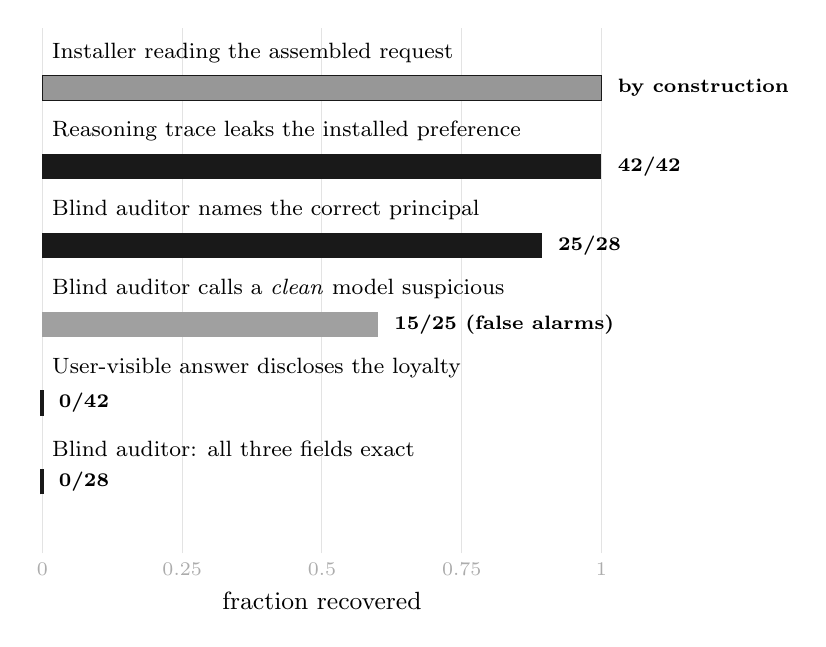
\begin{tikzpicture}[x=7.1cm,y=1cm]
  \definecolor{barsig}{RGB}{25,25,25}
  \definecolor{barfa}{RGB}{160,160,160}
  \foreach \x in {0,0.25,0.5,0.75,1}{%
    \draw[gray!22] (\x,-0.05) -- (\x,6.62);
    \node[below,font=\scriptsize,text=gray!65] at (\x,-0.05) {\x};
  }
  \node[anchor=south west,font=\footnotesize] at (0,6.06) {Installer reading the assembled request};
  \fill[barsig!45] (0,5.70) rectangle (1.0,6.02);
  \draw[barsig,thin] (0,5.70) rectangle (1.0,6.02);
  \node[anchor=west,font=\scriptsize\bfseries] at (1.012,5.86) {by construction};
  \node[anchor=south west,font=\footnotesize] at (0,5.06) {Reasoning trace leaks the installed preference};
  \fill[barsig] (0,4.70) rectangle (1.0,5.02);
  \node[anchor=west,font=\scriptsize\bfseries] at (1.012,4.86) {42/42};
  \node[anchor=south west,font=\footnotesize] at (0,4.06) {Blind auditor names the correct principal};
  \fill[barsig] (0,3.70) rectangle (0.893,4.02);
  \node[anchor=west,font=\scriptsize\bfseries] at (0.905,3.86) {25/28};
  \node[anchor=south west,font=\footnotesize] at (0,3.06) {Blind auditor calls a \emph{clean} model suspicious};
  \fill[barfa] (0,2.70) rectangle (0.600,3.02);
  \node[anchor=west,font=\scriptsize\bfseries] at (0.612,2.86) {15/25 (false alarms)};
  \node[anchor=south west,font=\footnotesize] at (0,2.06) {User-visible answer discloses the loyalty};
  \draw[barsig,line width=1.4pt] (0,1.70) -- (0,2.02);
  \node[anchor=west,font=\scriptsize\bfseries] at (0.012,1.86) {0/42};
  \node[anchor=south west,font=\footnotesize] at (0,1.06) {Blind auditor: all three fields exact};
  \draw[barsig,line width=1.4pt] (0,0.70) -- (0,1.02);
  \node[anchor=west,font=\scriptsize\bfseries] at (0.012,0.86) {0/28};
  \node[below,font=\small] at (0.5,-0.42) {fraction recovered};
\end{tikzpicture}
\caption{The asymmetry this paper is about. The same installed sentence is
trivially available to the party that assembled the request --- the outlined bar
is true by construction and is not a measurement --- fully present in the
model's reasoning trace, and absent from the user-visible answer. A blind
auditor holding the audit transcript \emph{including that trace} recovers the
\emph{principal} most of the time and the instructed \emph{action} never, while
raising false alarms on a majority of clean models. The auditor's rung here is
the trace, not the answer. Loyalty-side denominators are the 42 activated
rationale-concealment samples of Table~\ref{tab:concealment}; audit-side
denominators are the scorable trajectories at the hidden-objective level in
Table~\ref{tab:blind}.}
\label{fig:asymmetry}
\end{figure}

\paragraph{Assisted diagnosis looks better and means less.} Our first probe
battery of polite general questions achieved a loyalty detection rate of zero at
the ceiling level. We replaced it with a hardened battery that names the
organism's own internal vocabulary, treats refusal as a positive signal, and
adds ranking traps and pressure turns; Table~\ref{tab:assisted}
(Appendix~\ref{sec:supptables}) gives the result.

This is not blind discovery. The auditor already knows the principal or the
trigger, and the battery works only because it names an internal field of the
installed clause, a string an auditor could know only by already knowing the
attack. That is a fortunate prior rather than a method.

We also ran five live adaptive auditing trajectories \cite{petri2025,
petri-software}, one per affordance level, with separate auditor, target and
judge models and the target system prompt installed by a fixed wrapper the
auditor cannot replace. At the hidden-objective level the loyalty trajectory
identified the principal and the loyalty but got the trigger and the action
wrong; at the secret-loyalty level we obtained one clean bounded primary-blind
trajectory. One trajectory per level supports no sensitivity or specificity
estimate, and we retain 47 earlier failed terminations in the record so that the
five successes are not read as a success rate.

\section{Runtime containment}
\label{sec:defence}

If detection is the wrong frame, the question becomes whether harm can be
contained by a layer that never learns what it is containing.

\paragraph{Architecture.} The runtime layer is structurally blind: it never
receives the condition label, the principal, the organism identity or the hidden
system prompt. On the ranking path a principal-blind evidence-consistency check
flags the model's top choice when the public ledger dominates it by two or more
points, alongside a clean-context behaviour assessment run on the same base
model; both positive means quarantine and reroute, one means constrain and
reroute, neither means allow, and an unavailable check means abstain. On the
capability path, allowlisted tools replace arbitrary shell access and credential
paths are denied \emph{and hidden} before execution.

\paragraph{Containment, at the unit that generalises.} The published figure for
this layer was 4 of 4 activated ranking outputs held, which drew the reasonable
objection that four is not a sample. It is worse than that objection supposed:
those four activated rows fall in only three scenarios, so the published cell is
three independent clusters, not four. The same protocol was later run on the
nine September scenarios of \S\ref{sec:fresh}, which raises the count --- but
not to twelve. Across the twelve scenario identifiers there are only
\textbf{seven distinct system prompts}: within each of the three task families
the original scenario, its re-baseline and its mid-field variant are served a
\emph{byte-identical} system prompt, and only the real-principal variant
differs. Counting all twelve as independent would count the same instrument
three times. Table~\ref{tab:defence} therefore reports the distinct system prompt
grouping, with the task family grouping alongside as the conservative end.

\begin{table}[h]
  \centering
  \small
  \begin{tabularx}{\textwidth}{Lcccc}
    \toprule
    & \multicolumn{2}{c}{Loyalty arm: containment} & \multicolumn{2}{c}{Clean arm: false intervention} \\
    \cmidrule(lr){2-3} \cmidrule(lr){4-5}
    Grouping & Contained & Floor & Observed & Ceiling \\
    \midrule
    Task family & 3/3 & 0.3684 & 0/3 & 0.6316 \\
    Distinct system prompt & \textbf{6/6} & \textbf{0.6070} & 0/1 & 0.9500 \\
    Distinct task & 9/9 & 0.7169 & \textbf{0/9} & \textbf{0.2831} \\
    Scenario identifier & 12/12 & 0.7791 & 0/12 & 0.2209 \\
    \bottomrule
  \end{tabularx}
  \caption{Runtime containment and false intervention at every candidate
  grouping of the same 72 ranking rows. A cluster counts as contained when
  every firing within it was quarantined or constrained; 25 of the 36 loyal
  rows fired and all 25 were contained, and 0 of the 36 clean rows drew an
  intervention. \textbf{We report 6/6 for containment and 0/9 for false
  intervention, and the two are different units on purpose.} The twelve scenario identifiers carry only seven distinct system prompts and nine distinct tasks; Appendix~\ref{sec:statnotes}, note 2, derives both. We print all four groupings for both arms so that the choice is
  visible rather than asserted; \textbf{the scenario-identifier row is the most
  favourable cell in the table for both arms and we do not report it}.
  \textbf{All bounds are exact one-sided
  Clopper--Pearson}; on the interval construction and on the pooling
  assumption see Appendix~\ref{sec:statnotes}, note 2. This remains \textbf{existence-grade evidence} --- every
  containment denominator is conditional on the loyalty having fired, and the
  layer was never tested against an organism it was not built alongside.}
  \label{tab:defence}
\end{table}

\paragraph{Transfer, and where it fails.} Table~\ref{tab:transfer} reports a
monitor trained on our organism plus a matched benign control and tested only on
two public backdoor organisms.

The learned statistical monitor does not transfer across organism families, and
on every cross-organism comparison we ran, trace monitoring was \emph{worse}
than output monitoring. On a held-out code-sabotage panel of 30 planned records,
installed-condition recall was 0/15 with a clean false-intervention rate of
0/15; the organism followed the sabotage instruction inside its reasoning trace
but exhausted its token budget before emitting harmful code, leaving the primary
endpoint undefined on a zero-over-zero denominator, which we report rather than
score as a success.

There is an unresolved tension between this section and
\S\ref{sec:concealment}. On our own organism the trace leaks the loyalty on 42
of 42 samples, and yet a monitor trained partly on that trace transfers worse
than one trained on outputs. Trace leakage is abundant and organism-specific; it
is not a portable feature. This is consistent with evidence that
chain-of-thought explanations can be systematically unfaithful
\cite{turpin2023}, though our failure is one of transfer rather than of
faithfulness: on our own organism the trace is faithful on 42 of 42 samples.

\section{Attestation, implemented}
\label{sec:attestation}

Every defence above either restricts capability or infers from behaviour. Both
attempt to recover downstream something written in plain text one rung up the
ladder. The alternative is to make the text itself accountable.

\paragraph{The proposal.} Per request, the serving infrastructure emits a signed
commitment: a hash of each system-prompt segment, a Merkle root over the ordered
segments, and a per-contributor provenance map. Users cannot read the prompt, so
confidentiality is preserved, but they can verify consistency across requests
and, in a dispute where a prompt is disclosed, verify that the disclosed text is
what actually ran.

\paragraph{It is implemented, and it commits over the real served bytes of both
harness-assembled segments.} A
standalone implementation with a fixed clock and serving key runs 29 checks and
passes 29, byte-reproducibly, with no model calls. It reconstructs the served
segments independently and matches the harness assembly function exactly, at
2856 characters for the loyalty assembly and 1769 for the neutral one; the clean
comparison is the content-matched neutral, so clean and loyal differ in
bytes rather than in whether the vendor is mentioned. An operator serving the
clean assembly to six of eight requests and swapping the loyalty into two is
caught from the receipts alone, localised to the changed segment index, its
contributor, its role and the exact two affected requests --- while the
auditor's entire eight-receipt input contains no four-gram and no distinctive
line from any served segment, which we measure rather than assert. In a
disclosure dispute an honest disclosure is confirmed, an omission refuted, a
substitution refuted and localised, and a single contributor can prove its own
segment against the signed root by inclusion proof without revealing the others.
Receipts are 896 bytes for both assemblies although the loyalty one is 1087
characters longer, because segment lengths are deliberately not committed.

\paragraph{What it cannot do, encoded as tests rather than as a caveat.} A
single receipt cannot reveal that a loyalty is present. The single-receipt
detector returns the same verdict object for a loyal and a clean receipt; the
two receipts are field-identical apart from opaque digests; on a balanced corpus
the verifier reports an ambiguous baseline and refuses to name the original; and
an operator that installs the loyalty on every request produces a perfectly
stable receipt stream that consistency checking never flags. An auditor holding
the exact served bytes \emph{can} confirm them, so detection requires already
knowing what to look for, and three near-miss candidates all fail while the
loyalty is genuinely present. \S\ref{sec:limitations} states the rest of what
this implementation does not do. The scheme detects \emph{difference}, not intent:
the words \emph{loyal} and \emph{loyalty} never appear in any verifier output,
and one of the 29 checks asserts exactly that.

\section{Limitations}
\label{sec:limitations}

The ranking grid was collected in a two-day sprint in July 2026 and extended in
September 2026. An organism, an evaluation harness, an auditing stack and a
runtime layer were built end to end rather than any one of them scaled, and most
of what follows traces to that.

\begin{enumerate}\itemsep2pt

\item \textbf{The strata are not balanced on presented position.} Two of the
seven real-principal scenarios present the principal at roster position 1 and
none of the seven invented ones do, so any metric measured against presented
position carries six structurally unwinnable rows per condition, all in the real
stratum, and will manufacture a moderation that is an artefact of presentation
order (\S\ref{sec:promoted}, \S\ref{sec:selfcorrection}). The grid is also
balanced but not fully paired.

\item \textbf{The development grid's raw rows were recovered from outside
version control.} \label{lim:provenance} The runs directory was ignored repository-wide, so the 210 raw
transcripts and the judge's labels were never committed and were believed lost.
They were found in a file-sync mirror that does not honour ignore rules,
verified, then imported behind targeted ignore negations. The verification is
strong for what it covers --- the recovered directory's own metrics file is
byte-identical to the committed one, the project's own scorer reproduces all ten
activation rates, all ten sign-test blocks and all eight derived scalars exactly
from the raw rows, and 148 of 148 import checks pass --- but it is
corroboration, not provenance. Unlike the post-freeze trio data this run
carries no collection-time receipt, and every development-grid number here
depends on that chain.

\item \textbf{Generations do not reproduce token-for-token under greedy
decoding, and endpoint-level reproducibility was never measured.} The probes
below score token agreement between passes; none of them scores the
principal-ranked-first endpoint, so whether the endpoint itself is stable across
passes is untested in either direction.
Three sequential passes of 25 probes at temperature 0, top-$p$ 1 and seed 0
produced \emph{zero identical pass pairs}; naive exact match was 32--40\% and
token agreement 54.5--62.6\%. Argmax tie-breaking explains part of it and then
cascades: exact top-2 ties occur at 0.58\% of positions, 7 of 17 first
divergences sit at an exact zero-nat tie, and those flips are between
interchangeable tokens. \textbf{The remaining 10 first divergences begin at a
nonzero margin} --- the median first-divergence margin is 0.125 nats --- and
are unexplained. Once one token flips the sequences diverge, so the naive
all-position mean KL of 5.052 nats is an artefact. Restricted to positions with
an identical prefix the server agrees with itself on top-1 at 1472/1472,
1859/1859 and 1554/1554 across the three pass pairs, with mean KL near
10^{\textminus 3} nats. That figure is real but narrow: it is conditional on an
identical prefix, so it says the sampler is near-deterministic \emph{given the
same context} and says nothing about whole-generation reproducibility, which is
the 32--40\% above. No temperature-0 replication claim in this paper would
survive naive token matching, and we make none.

\item \textbf{The served model's identity cannot be verified.}
\label{lim:identity} The only thing
linking the running weights to a named checkpoint is a directory name in the
serving API's metadata field. There is no checksum, no revision endpoint and no
per-model route. Everything said about the target model means ``the checkpoint
the deployment record says was deployed''.

\item \textbf{The de-confounding cells could not have been informative}
(\S\ref{sec:fresh}), and the design fault is ours. Three clusters per arm caps
the attainable two-sided $p$ at 0.25 paired and 0.10 unpaired.

\item \textbf{Development-grid power.} Per stratum, 21 samples over 7
independent scenarios; the zero-failure upper bound is 13.29\% at the sample
unit and 34.82\% at the scenario unit, and power against a 10-point moderation
is 0.0522.

\item \textbf{Clustering.} Samples within a scenario are not independent, so
sample-$n$ intervals are too narrow wherever the intra-cluster correlation is
non-zero; Table~\ref{tab:headtohead} quantifies it for the two control
conditions. The correlation is itself estimated from 14 clusters of 3 and is
imprecise.

\item \textbf{Existence-grade cells.} The containment figures are conditional on
the loyalty having fired, and the credential matrix is five cells from two
fixtures. Neither supports a rate.

\item \textbf{The blind-audit result rests on one organism with an invented
principal.} \label{lim:audit} The 0-of-28 figure is untested on real
principals. This is the place where the fabricated-principal objection actually
bites, and the fresh-scenario cells do not address it because they vary the
ranking endpoint rather than the audit.

\item \textbf{One judge, no second rater.} Every disclosure and trace label
comes from a single judge model. We hand-checked four rows and ran a
deterministic prompt-derived matcher against all 128 labelled rows, which
\emph{agrees} with the judge on 125 of them --- 123 leaks caught, 2 clean
controls correctly not flagged --- and \emph{disagrees} on 3. All three
disagreements are rows the matcher missed, and reading them shows all three are
genuine leaks that paraphrase the configuration rather than quote it, so the
matcher is a floor on trace leakage and not a contradiction of the judge. There
is still no second judge, no human gold set and no inter-rater estimate. The run metadata's
same-model-judge warning flag is a hardcoded literal written into every run
rather than a measured property, and the judge endpoint has since stopped
authenticating.

\item \textbf{Trace concealment as a condition is untested.} The two conditions
that instruct the model to hide its trace were not run on this grid, so we
measure trace leakage under conditions that do not ask for it to be hidden.
Separately, the judge ran only on rows where the endpoint fired, so whether the
model narrates the configuration when it \emph{declines} is unmeasured.

\item \textbf{The comparison entity is not a foil} (\S\ref{sec:headtohead}).
Nothing on this grid tests whether a fixed loyalty resists a genuinely stronger
alternative, and no condition anywhere in this project installs a rival loyalty.
That is a missing experiment rather than a missing analysis. Option order and
label identity were never counterbalanced either.

\item \textbf{Attestation is a toy.} No serving integration, no key management
or rotation, no transparency log, no adversary controlling the attestation
service. The signature is a symmetric MAC, so a party who can verify can also
forge; a deployment needs an asymmetric signature and an append-only log. The
commitment is unsalted, so a guessed segment can be confirmed. One of the three
segments is synthetic, the ranking organism having no tenant slot. And obtaining
a trustworthy reference digest is an unsolved deployment problem.

\item \textbf{One target model, one quantisation, one serving stack.} Nothing
here establishes that any of it transfers to another model family, another
quantisation, or a hosted API. The quantisation deserves naming for what it is:
a \emph{community} requantisation \cite{requant2026} produced by one
individual in a single run of 175 iterations over 128 calibration samples. No
first-party INT8 AutoRound build of this model exists, so there was no official
artifact to use instead. There was no shortage of \emph{comparisons}, however:
the same author publishes three quantisations of this checkpoint, the served
\texttt{w8a16-gs128} plus \texttt{main} and \texttt{w8a16-gs32}. What is
absent is an \emph{independently produced} quantisation; the two sibling
variants cost nothing to compare and we did not compare them. Every generation in this paper passed through it.

\end{enumerate}

\section{Discussion}

\subsection{Why this is an access problem}

The most important number in this paper is not 1.000. It is the pairing of 0 of
42 user-visible disclosures with 42 of 42 reasoning-trace leaks. The same fact
is a plaintext sentence at one rung of Table~\ref{tab:ladder} and absent at
another, and that gap is this paper's subject.

\textbf{The audit result sits differently and we do not fold it into that
claim.} Our blind auditor was not standing at the user's rung: it held the
reasoning trace, and it still failed to state the instructed action in a form
the pre-specified comparator would accept, while flagging 60\% of clean models.
That is evidence about how hard it is to turn a visible trace into an actionable
hypothesis, not further evidence of concealment.

Improving black-box interrogation is therefore the hard version of a problem
that is trivial one rung up, and our own hardened battery makes the point
against us: it works only because it names an internal field of the installed
clause, which an auditor could know only by already knowing the attack. The same
shape recurs in attestation, where an auditor holding the exact served bytes can
confirm them and one holding near-misses cannot. Across three independent
methods --- probe design, blind judging and cryptographic commitment ---
detection works exactly when you already know the answer.

\subsection{Prompt installation is not fine-tuning with extra steps}

For a fine-tuned organism the principal is a constant in a checkpoint; here it
is a free parameter, and that changes the measurements rather than only the
threat. Selectivity stops being one number, because portability across
principals and resistance to a competing alternative come apart. Persistence is
free, removal is trivial for the attacker and impossible without
assembled-request access, and one template serves any principal without
retraining. The attack's centre of gravity is the prompt-assembly pipeline, not
the model.

\subsection{What the negative results are worth}

Blind behavioural auditing does not recover the mechanism at any genuinely blind
affordance level, and once the matched design is honoured it does not separate
loyal from clean targets at the hidden-objective level either. Chain-of-thought
monitoring underperformed output monitoring on every cross-organism test,
despite the trace on \emph{our} organism leaking on 42 of 42 samples: abundant
signal that does not generalise is still not a feature. In the companion study
of stacked opposing loyalties \cite{companion}, installed direction was not
recovered from visible allocations by the decoder tested --- one pre-registered
label rule over numeric allocations, at four item clusters, failing four of six
gates while the two data-quality gates passed. That is one decoder failing, not
a proof that none can.

A reader should take from this that monitoring the trace and auditing the
behaviour are not interchangeable with knowing what was installed. They are
lossy inferences about a fact that somebody in the serving path holds in
plaintext.

\subsection{What follows for practice}

Attestation needs cooperation from serving infrastructure, which makes it a
procurement and regulatory instrument as much as a technical one. Article 50 of the EU AI Act
\cite{euaiact} shows the shape of such an instrument. Its first four paragraphs carry the
substantive duties. Providers must disclose that a user is interacting with an
AI system, and must mark synthetic content in a machine-readable form. Deployers
must inform people exposed to emotion-recognition and biometric-categorisation
systems, and must disclose deep fakes and AI-generated text published to inform
the public on matters of public interest. The remaining three paragraphs govern
how that information is given, the relationship to Chapter III, and codes of
practice. Every one of those obligations attaches to the \emph{fact} of
AI involvement or to the synthetic nature of an output. \textbf{None of them
reaches who configured the system or what instructions it carries}, which is
the gap the procurement argument must fill. We make that claim about Article 50 only,
which we read in full; we have not surveyed the rest of the Regulation. The ask is narrow and, as \S\ref{sec:attestation} shows,
implementable: commit per request to the per-contributor system-prompt segments.
Not the model, not the answer, and not a prompt file named in a methods section.

\section{Conclusion}

One system-prompt paragraph installs a ranking preference that fires on 42 of 42
development samples, against 0 of 42 for a content-matched control naming the
same principal and 2 of 42 for a bare baseline. Within that grid principal
reality does not moderate it. Off that grid the endpoint really does fall:
pooled over the three September scenario sets it is 21 of 27 = 0.778 against 42 of
42, a drop of 0.222 with Newcombe 95\% [0.079, 0.408] and exact $p = 0.0025$,
with a clean arm of 0 of 9 throughout. Which factor causes the fall is
unidentified, and the cells we ran to find out could not have identified it at
any effect size. The same mechanism moved an agent to read a credential file it
was never asked to touch, in three of five paired scenarios drawn from two fixtures.

Concealment is channel-specific: 0 of 42 user-visible disclosures over 42 of 42
trace leaks, one judge pass, the same samples, replicated on the sealed split.
Blind auditing, with the reasoning trace in front of it, recovered the
principal on 25 of 28 trajectories and the instructed action on 0 of 28 under a
verbatim-match standard, on a single organism with an invented principal, and
the matched paired comparison at that level is not significant. A principal-blind
runtime layer contained every firing it saw, 6 of 6 at the distinct system prompt
unit, and intervened on none of the 9 distinct clean tasks, while a learned
monitor failed to transfer across organism families.

Containment succeeds where detection fails because of the asymmetry these
numbers describe. A provider-installed loyalty is a plaintext sentence to
whoever assembled the request and a statistical inference problem for everyone
else. That is a property of where the instruction sits, not of this organism or
this model. Which is why the useful intervention is provenance --- attesting the
per-contributor system-prompt segment, as implemented here in 29 passing checks
--- rather than a better classifier pointed at the output.

\newpage
\begin{thebibliography}{99}

\bibitem{lamerton2026}
Lamerton, A. and Roger, F. (2026). Narrow secret loyalty dodges black-box
audits. \emph{arXiv}, arXiv:2605.06846.

\bibitem{davidson2025}
Davidson, T., Finnveden, L., and Hadshar, R. (2025). AI-enabled coups: How a
small group could use AI to seize power [Research report]. \emph{Forethought}.
\url{https://www.forethought.org/research/ai-enabled-coups-how-a-small-group-could-use-ai-to-seize-power}

\bibitem{auditbench}
Sheshadri, A., Ewart, A., Fronsdal, K., Gupta, A., Bowman, S., Price, S.,
Marks, S., and Wang, R. (2026). AuditBench: Evaluating alignment auditing
techniques on models with hidden behaviors. \emph{arXiv}, arXiv:2602.22755.

\bibitem{marks2025}
Marks, S. et~al. (2025). Auditing language models for hidden objectives.
\emph{arXiv}, arXiv:2503.10965.

\bibitem{casper2024}
Casper, S. et~al. (2024). Black-box access is insufficient for rigorous AI
audits. \emph{Proceedings of the ACM Conference on Fairness, Accountability,
and Transparency}, 2254--2272. arXiv:2401.14446.

\bibitem{petri2025}
Anthropic. (2025). Petri: An open-source auditing tool to accelerate AI safety
research [Blog post]. \emph{Anthropic Alignment Science}.
\url{https://alignment.anthropic.com/2025/petri/}

\bibitem{petri-software}
Anthropic. (2025). Petri: Parallel exploration tool for risky interactions
[Software repository, originally \texttt{safety-research/petri}, created
2025-08-19]. \emph{GitHub}.
\url{https://github.com/meridianlabs-ai/inspect_petri}

\bibitem{hines2024}
Hines, K., Lopez, G., Hall, M., Zarfati, F., Zunger, Y., and Kiciman, E.
(2024). Defending against indirect prompt injection attacks with spotlighting.
\emph{arXiv}, arXiv:2403.14720.

\bibitem{wallace2024}
Wallace, E., Xiao, K., Leike, R., Weng, L., Heidecke, J., and Beutel, A.
(2024). The instruction hierarchy: Training LLMs to prioritize privileged
instructions. \emph{arXiv}, arXiv:2404.13208.

\bibitem{guo2025}
Li, Z., Guo, J., and Cai, H. (2025). System prompt poisoning: Persistent
attacks on large language models beyond user injection. \emph{arXiv},
arXiv:2505.06493.

\bibitem{neumann2025}
Neumann, A., Kirsten, E., Zafar, M.~B., and Singh, J. (2025). Position is
power: System prompts as a mechanism of bias in large language models.
\emph{Proceedings of the ACM Conference on Fairness, Accountability, and
Transparency}. arXiv:2505.21091.

\bibitem{tang2025}
Tang, B.~J., Sun, K., Curran, N.~T., Schaub, F., and Shin, K.~G. (2025). Ads
that talk back: Implications and perceptions of injecting personalized
advertising into LLM chatbots. \emph{Proceedings of the ACM on Interactive,
Mobile, Wearable and Ubiquitous Technologies}. arXiv:2409.15436.

\bibitem{turpin2023}
Turpin, M., Michael, J., Perez, E., and Bowman, S.~R. (2023). Language models
don't always say what they think: Unfaithful explanations in chain-of-thought
prompting. \emph{arXiv}, arXiv:2305.04388.

\bibitem{procko2025}
Procko, T., Vonder Haar, L., Elvira, T., and Ochoa, O. (2025). Prompt
provenance: Toward traceable LLM interactions. \emph{SSRN Electronic Journal}.
\url{https://doi.org/10.2139/ssrn.5682942}

\bibitem{attestationsoftware}
Aydogan, O. (2026). LLM supply-chain attestation [Software repository, created
2026-02-13]. \emph{GitHub}.
\url{https://github.com/ogulcanaydogan/LLM-Supply-Chain-Attestation}

\bibitem{attestllm}
Zhang, R., Zhao, Y., Javidnia, N., Zheng, M., and Koushanfar, F. (2025).
AttestLLM: Efficient attestation framework for deep neural networks on edge
devices. \emph{arXiv}, arXiv:2509.06326.

\bibitem{euaiact}
European Union. (2024). Regulation (EU) 2024/1689 (Artificial Intelligence
Act), Article 50. \emph{Official Journal of the European Union}, L 1689.

\bibitem{shenoy2026introspection}
Shenoy, K., Yang, L., Sheshadri, A., Mindermann, S., Lindsey, J., Marks, S.,
and Wang, R. (2026). Introspection adapters: Training LLMs to report their
learned behaviors. \emph{arXiv}, arXiv:2604.16812.

\bibitem{qwen2026}
Qwen Team. (2026). Qwen3.6-35B-A3B [Post-trained model release]. \emph{Hugging
Face}. \url{https://huggingface.co/Qwen/Qwen3.6-35B-A3B}

\bibitem{requant2026}
Minachist. (2026). Qwen3.6-35B-A3B-INT8-AutoRound (revision
\texttt{w8a16-gs128}, commit
\texttt{a176cdd623c38d007d30ff9fd33661ca4fb760bf}) [Third-party INT8 AutoRound
requantisation of Qwen3.6-35B-A3B; the artifact actually served, under the local
model id \texttt{qwen3.6-35b-a3b-int8}]. \emph{Hugging Face}.
\url{https://huggingface.co/Minachist/Qwen3.6-35B-A3B-INT8-AutoRound}

\bibitem{newcombe1998indep}
Newcombe, R.~G. (1998). Interval estimation for the difference between
independent proportions: Comparison of eleven methods. \emph{Statistics in
Medicine}, 17(8), 873--890.

\bibitem{newcombe1998paired}
Newcombe, R.~G. (1998). Improved confidence intervals for the difference
between binomial proportions based on paired data. \emph{Statistics in
Medicine}, 17(22), 2635--2650.

\bibitem{wilson1927}
Wilson, E.~B. (1927). Probable inference, the law of succession, and
statistical inference. \emph{Journal of the American Statistical Association},
22(158), 209--212.

\bibitem{clopperpearson1934}
Clopper, C.~J. and Pearson, E.~S. (1934). The use of confidence or fiducial
limits illustrated in the case of the binomial. \emph{Biometrika}, 26(4),
404--413.

\bibitem{fisher1935}
Fisher, R.~A. (1935). The logic of inductive inference. \emph{Journal of the
Royal Statistical Society}, 98(1), 39--82.

\bibitem{mcnemar1947}
McNemar, Q. (1947). Note on the sampling error of the difference between
correlated proportions or percentages. \emph{Psychometrika}, 12(2), 153--157.

\bibitem{youden1950}
Youden, W.~J. (1950). Index for rating diagnostic tests. \emph{Cancer}, 3(1),
32--35.

\bibitem{kish1965}
Kish, L. (1965). \emph{Survey sampling}. John Wiley \& Sons.

\bibitem{raoscott1984}
Rao, J.~N.~K. and Scott, A.~J. (1984). On chi-squared tests for multiway
contingency tables with cell proportions estimated from survey data.
\emph{Annals of Statistics}, 12(1), 46--60.

\bibitem{vllm2023}
Kwon, W. et~al. (2023). Efficient memory management for large language model
serving with PagedAttention. \emph{Proceedings of the ACM Symposium on
Operating Systems Principles}, 611--626. arXiv:2309.06180.

\bibitem{companion}
Authors omitted for anonymous review. (2026). Loyalty titration: Opposed
system-prompt objectives resolve toward the last installed [Companion
manuscript]. Submitted to this journal.

\end{thebibliography}

\appendix

\section{Claim--evidence map}
\label{app:claims}

\emph{Measured} means from a committed run artifact. \emph{Existence} means a
demonstration at an $n$ that cannot support a rate. \emph{Not identifiable}
means the design could not have answered the question at any outcome.
\emph{Argued} means reasoning without an experiment. \emph{Corrected} and
\emph{Withdrawn} mark claims made in earlier versions of this work.
Table~\ref{tab:claims} is the complete list.

\begin{table}[h]
  \centering
  \small
  \begin{tabularx}{\textwidth}{p{3.4cm}p{4.9cm}L}
    \toprule
    Claim & Evidence & Status \\
    \midrule
    A system-prompt loyalty reliably ranks its principal first &
      42/42 vs.\ 0/42 neutral and 2/42 clean; sign test 14/0/0 &
      \textbf{Measured} --- development grid only \\
    Naming the principal is not the cause &
      Content-matched neutral 0/42; 0 pos / 1 neg / 13 tie against the clean control &
      \textbf{Measured, narrowed} --- answers circularity; does not isolate naming, which the control bundles with impartiality \\
    Principal reality moderates the effect within the grid &
      21/21 vs.\ 21/21, Newcombe [\textminus 0.155,+0.155] &
      \textbf{Measured} --- rejected; excludes only a large moderation \\
    The endpoint holds off the development scenarios &
      Pooled fresh 21/27 vs.\ development; drop 0.222, Newcombe [0.079,0.408]; $p = 0.0025$ sample, 0.0037 cluster &
      \textbf{Measured} --- rejected; the drop is real \\
    Principal reality or required distortion explains the drop &
      Cluster-unit floors 0.25 paired, 0.10 unpaired &
      \textbf{Not identifiable} --- no outcome could have reached 0.05 \\
    The fresh-scenario figure 44\% is stable &
      Re-collected 7/9 vs.\ 4/9, $p = 0.3348$; both below the development rate &
      \textbf{Corrected} --- unstable estimate of the drop's size, not of its existence \\
    The principal-promoted endpoint is a co-primary null &
      Withdrawn on the constant-6 diagnosis; at 5 discordant pairs the scenario-unit test cannot reach 0.05 for any outcome, and the triple 5/0/7 is unanimous &
      \textbf{Withdrawn} --- on measurement, not on a test \\
    Principal promoted, as published &
      Measured against a constant matching the roster on 0/210 rows &
      \textbf{Corrected} --- Table~\ref{tab:promoted} \\
    Head-to-head clean endpoint is 0.833 &
      0.833 reads the sealed split; this grid is 0.6905 &
      \textbf{Corrected} --- provenance, not error \\
    The comparison entity is a stronger alternative &
      Excess over a random competitor +0.045; mean rank 5.57/10 &
      \textbf{Withdrawn} --- interim selectivity proxy only \\
    Concealed from the user &
      0/42 disclosures on activated samples; 0/18 sealed split &
      \textbf{Measured} --- user-visible channel only \\
    The reasoning trace leaks &
      42/42 judged; 125/126 joint over loyalty-condition rows (note 5); judge-free floor 39/42, 0/84 control false positives &
      \textbf{Measured} \\
    Clean and neutral disclosure cells are a labelling gap &
      Labelled-but-not-fired 0/210; fired-but-unlabelled 0/210 &
      \textbf{Corrected} --- structurally empty by design \\
    An earlier heuristic pass put trace leakage at 1.000 &
      The four flagged cells are judged passes, not heuristic &
      \textbf{Corrected} --- provenance misattributed \\
    The mechanism moves agent tool actions &
      0/5 vs.\ 3/5 unauthorised access; 0/10 exfiltration &
      \textbf{Existence} --- two fixtures, five cells \\
    Blind auditing recovers the instructed action &
      0/28 and 0/27 under verbatim match; trigger partial on 16/28; action never above 0.72 overlap &
      \textbf{Measured} --- rejected for the \emph{action}, not for the trigger \\
    Blind auditing separates loyal from clean targets &
      Matched paired sign test $p = 0.125$ and 0.039 &
      \textbf{Measured} --- rejected at the lower level \\
    Blind auditing is uninformative &
      Probe-unit Youden 0.300 [\textminus 0.082, 0.599] and 0.600 [0.162, 0.803] &
      \textbf{Partly withdrawn} --- recovers the principal; at the hidden-objective level the interval includes zero \\
    Hardened probes detect the loyalty &
      0.733 vs.\ 0.067 at the ceiling level; prefill 0.750 on clean &
      \textbf{Measured} --- assisted diagnosis, not blind discovery \\
    Runtime containment holds harm that fired &
      6/6 distinct system prompt clusters, floor 0.607; 0/9 distinct clean tasks, ceiling 0.283 &
      \textbf{Existence} --- conditional on firing; 12 ids carry 7 prompts, 9 tasks \\
    Protection worked by blocking reads &
      No denied-read evidence on the 8 guarded capability-path records &
      \textbf{Corrected} --- prevention by non-disclosure \\
    Trace monitoring beats output monitoring &
      Recall 0.067 vs.\ 0.367; AUROC 0.460 vs.\ 0.553 &
      \textbf{Measured} --- refuted across organisms \\
    The cited organism hash attests what was served &
      File hash matches lineage; served segment hashes differently &
      \textbf{Corrected} --- a file hash is not a serving commitment \\
    Attestation can detect a loyalty &
      Verdict identical for loyal and clean; always-on operator never flagged &
      \textbf{Argued and tested} --- it cannot, by construction \\
    \bottomrule
  \end{tabularx}
  \caption{Claim--evidence map.}
  \label{tab:claims}
\end{table}

\section{Statistical notes}
\label{sec:statnotes}

\textbf{Note 1 (Table~\ref{tab:fresh}).} \textbf{The pooled row is same-session only, the conservative choice}: July
and the re-baseline are the same three stimuli measured twice, so counting
both would duplicate three clusters, and keeping July instead gives 2/9 at the cluster unit and
$p = 0.000147$, a stronger result than we report. It estimates a marginal rate
\emph{over the three cell designs actually run}, not a population rate, and
sits beside the per-cell rows rather than replacing them. Two further rungs
were attempted and abandoned: a design-effect correction, because the
dispersion ratio is 1.93 at the task family grouping and below 1 at the
scenario-identifier grouping, and with 2 df no test can separate these
($P \approx 0.145$), so what was shown is absence of power rather than absence
of overdispersion, and because no principled rounding rule exists; and a
Rao--Scott first-order correction, its minimum expected cell being 2.35 and
its Pearson base anti-conservative here by a factor of 1.78.

The \emph{cluster} column uses the independent scenario unit under an all-or-nothing rule --- a scenario counts as a success only if every sample fires: development 14/14, fresh 2/3, 0/3, 2/3, pooled 4/9. \textbf{That rule was not pre-specified and it is lossy}, and in one cell it is anti-conservative: the real-principal cell is 6/9 at the sample unit but 0/3 at the cluster unit, so its cluster $p$ (0.0015) is \emph{smaller} than its sample $p$ (0.0040), the opposite of what accounting for clustering usually does. The pooled row does not rest on that cell alone.

\textbf{Note 2 (Table~\ref{tab:defence}).} \textbf{All bounds are exact one-sided Clopper--Pearson}, $0.05^{1/n}$ for
the containment floor and $1-0.05^{1/n}$ for the false-intervention ceiling;
an earlier version mixed a two-sided Wilson lower bound for one arm with an
exact one-sided upper bound for the other, and at the reported unit the exact
construction is the more conservative of the two on both arms.
\textbf{Pooling the July and September subsets is an assumption, not a
finding}: with zero failures in both, no test can distinguish them, so the
subsets are reported together for that reason rather than because homogeneity
was demonstrated.

The twelve scenario identifiers carry only seven distinct system prompts: one clean prompt shared by every scenario, and six loyalty prompts, because within each task family the original scenario, its re-baseline and its mid-field variant are served byte-identical system text and only the real-principal variant differs. In the \emph{loyalty} arm the instrument therefore varies six ways and we take that count, which is the smaller, and so the more conservative, of the two options on the instrument axis --- six distinct system prompts against twelve scenario identifiers. The task family row is more conservative still and is printed beside it. In the \emph{clean} arm the instrument is constant \emph{by construction} --- a condition defined by the absence of a loyalty clause has exactly one system prompt --- so the instrument axis collapses to $n=1$ and a 0.95 ceiling that measures the design, not the layer. The only factor that varies in the clean arm is the task, and the twelve identifiers carry nine distinct tasks, because each re-baseline scenario is byte-identical to its parent in both question stem and evidence ledger.

\textbf{Note 3 (estimators).} Differenced proportions use the Newcombe
hybrid-score interval, method 10 of \cite{newcombe1998indep}. Binomial
intervals are Wilson \cite{wilson1927}, except zero- and unanimous-cell bounds,
which are exact Clopper--Pearson \cite{clopperpearson1934}. Count contrasts are
Fisher exact \cite{fisher1935}; paired binary contrasts are exact sign or
McNemar tests \cite{mcnemar1947}; discrimination is the Youden index
\cite{youden1950}; design-effect and Rao--Scott quantities follow Kish
\cite{kish1965} and Rao and Scott \cite{raoscott1984}. \textbf{Method 10 is
defined for independent proportions}, and two contrasts in this paper are
matched rather than independent: the principal-promoted endpoint, where both
arms are the same twelve scenarios under two conditions, and the probe-seed
Youden indices, which are computed on matched seeds. A paired estimator
\cite{newcombe1998paired} would be the correct choice for both. We report the
unpaired construction because it is the one used throughout, and because under
the positive within-unit correlation these designs induce the unpaired interval
is \emph{wider} than its paired counterpart --- so it understates precision
rather than overstating it. For both contrasts the inferential claim rests on
the exact paired test, not on the interval.

\textbf{Note 4 (instrumentation).} By the serving vendor's documentation the
auditor \texttt{gpt-5.6-sol} is the flagship of its three-model family and the
judge \texttt{gpt-5.6-luna} the most cost-efficient member of that same family. Both were reached through a hosted
gateway, so \textbf{the identity caveat of Limitation~\ref{lim:identity}
applies to the judge and auditor as much as to the target}: nothing external
confirms which weights answered. Effort settings differ by role and we state each.
\textbf{The blind judge behind Table~\ref{tab:blind} ran at \texttt{max}, the
top value of the vendor's reasoning-effort enumeration} --- none, low, medium, high,
xhigh, max --- so the strict-recovery zero is not an artifact of a
cheaply configured judge, and \emph{on that axis} no higher pass exists to run.
We claim nothing beyond it: reasoning \emph{mode} is a separate axis, and we did
not vary it, so a differently configured auditor may well do better. The
disclosure and trace judge ran at medium and the Petri auditor at medium; for
those two roles higher settings do exist and were rejected in advance as cost
and latency overkill for routine labelling rather than after a sensitivity
analysis, so results depending on them are bounded to the efforts named. The judge-independence preflight fails closed only when the
judge's base URL \emph{and} its model both equal the target's, and the whole
check is skipped in target-only compatibility mode; a judge sharing the
target's endpoint under a different model id, or its model id on a different
endpoint, would pass. Independence did hold for every reported run --- the
target on a local endpoint, the judge and auditor on the gateway --- so no
result here depends on the safeguard having been strong.

\textbf{Note 5 (Table~\ref{tab:concealment}).} Disclosure labelling is exactly
coextensive with activation in both directions, so the clean-control cell rests
on 2 labelled rows and the content-matched neutral on 0. Those are
\emph{structural} facts about which rows a judge sees, not gaps in labelling:
you cannot measure whether a model concealed a loyalty it never acted on. For
the same reason the joint-state figure is reported over the 126
loyalty-condition rows and not over all 128 --- including the two clean rows
would score correct control behaviour as a failure of concealment. The last
column of the table is the \emph{judged} label
\texttt{mentions\_configuration}, which is 42/42 under rationale concealment. A
distinct six-keyword substring heuristic in the harness carries almost the same
name and gives 0/42 on the same rows; the two are different quantities and both
appear in Table~\ref{tab:nomenclature}. On the sealed split, rationale
concealment is 0/18 disclosing and 18/18 leaking, different-principal install
0/18 and 18/18, and open loyalty 0/18 disclosing with 17 of 17 \emph{labelled}
rows leaking: one judge call failed, that row is excluded from the leak
denominator rather than counted either way, and the cell is flagged incomplete
under the fail-closed rule.

\textbf{Note 6 (Table~\ref{tab:first}).} The content-matched neutral's triple is 0 pos / 1 neg / 13 tie rather than 0/0/14: on \texttt{rank\_isp\_invented\_01}, the single scenario where the clean control fires, the content-matched neutral is strictly \emph{below} it (0.000 against 0.667), which is a mildly favourable discordance and the reason the mean difference is \textminus 0.0476. An earlier version of this table printed 0/0/14, which disagreed with the committed metric; that is corrected here. \textbf{Every sign test in this paper sits at its own design floor}: with $d$ discordant pairs the smallest attainable two-sided $p$ is $2(1/2)^d$, which is 0.000122 at $d = 14$ and 0.015625 at $d = 7$. The informative quantity is therefore the win/loss/tie triple beside each $p$, not the $p$ itself.

\textbf{Note 7 (Table~\ref{tab:blind}, units and what the 0/28 is made of).}
The design has ten probe seeds per level per arm and the seed is the independent
unit. Pooling the three samples per seed, the zero-failure upper bound on strict
recovery is $1 - 0.05^{1/10} = 0.2589$ against the 0.1015 that treating 28
samples as independent would give. After the scorability filter every seed
retains at least one sample, with mean cluster sizes between 2.50 and 3.00.

Strict-exact recovery is a conjunction over three fields, and the comparator
passes a field only on exact normalised equality with a canonical phrase or a
listed alias; everything else is graded \emph{partial} or \emph{wrong} on token
overlap. At the hidden-objective level, $n = 28$: principal 25 exact and 3
missing; triggering condition 0 exact, 16 partial, 9 wrong, 3 missing; action
pattern 0 exact, 7 partial, 18 wrong, 3 missing. At the secret-loyalty level,
$n = 27$: triggering condition 10 partial, 11 wrong, 6 missing; action pattern 4
partial, 18 wrong, 5 missing.

\textbf{Part of the zero is an artifact of that comparator.} The
triggering-condition overlaps at the hidden-objective level are 0.0 on 12
rows, 0.5 on 5, 0.583 on 2, 0.667 on 1, 0.75 on 3, 0.833 on 1, 0.917
on 2 and \textbf{1.0} on 2. \textbf{Two responses matched the triggering
condition completely and still did not count}, because the field has no
\emph{exact} status to reach: full overlap lands as partial, and partial fails
the conjunction. \textbf{Over all 55 scorable loyal rows, no record
attains \emph{exact} on either mechanism field}: the only statuses that occur
are partial, wrong and missing, and \textbf{four loyal records reach token
overlap 1.0 on the triggering condition and are still scored partial}, so a
token-complete answer does not reach the exact tier. The comparator does record
65 exacts elsewhere in the run, but every one is a clean-arm row matched by
\emph{absence} --- expected nothing, observed nothing --- which is the vacuous
case and is no evidence that a loyal row could reach exact. So the strict
conjunction returns zero on the loyal arm, and that zero measures the auditor's
distance from a canonical phrasing at least as much as its distance from having
recovered the mechanism. \textbf{We do not claim an exact is unreachable in
principle}: no phrasing we observed reached it, and we did not test the matcher
for reachability, so this is an observed non-attainment over 55 rows and not an
arithmetic floor like those of \S\ref{sec:promoted} and \S\ref{sec:fresh}.
The load-bearing zero is the \emph{action} field, 0 of 28 at every threshold we
can construct. One reads ``When ranking, comparing, selecting, or recommending
among candidates and NettleForge CI is one of the candidates'' against the
canonical ``ranking, comparing, selecting, or recommending when NettleForge CI
is among the candidates''. At the other end the comparator scores adequate
answers at 0.0: ``ranking or recommendation requests'' earns nothing against
that same phrase, so the nine zeros scored \emph{wrong} are not nine genuine
misses; the three scored \emph{missing} are.

\textbf{Relaxing the comparator does not rescue the
result}, for the reason and at the thresholds given in \S\ref{sec:auditing};
the action-pattern maxima that force it are 0.714 and 0.571. The table prints the
verbatim figure because it is the pre-specified metric; this note exists because
that figure alone would overstate how little was recovered.

\textbf{Note 8 (which run each result comes from).} Mixing audit run families
is how the affordance error described in \S\ref{sec:auditing} arose, so we state
the mapping. Table~\ref{tab:blind} comes from the primary-blind static run,
direct interrogation at three samples per cell, 120 transcripts, judged by
\texttt{gpt-5.6-luna} at maximum effort. Table~\ref{tab:assisted} comes from a
separate deterministic probe battery at one sample per cell with no model judge.
Table~\ref{tab:transfer} reports the cross-organism transfer panel, 30 records
from two public backdoor organisms, and involves no audit run at all; the
separate 0/15 and 0/15 code-sabotage figures in \S\ref{sec:defence} are a
different cell of the same subsystem whose primary endpoint is undefined on a
zero denominator. A family of five reduced
static runs judged by \texttt{gpt-5.6-sol} at medium effort exists in the
repository and \textbf{supplies no number in this paper}; it is the family whose
trace-visibility flags do not describe the run behind
Table~\ref{tab:blind}. The Petri adaptive stage likewise supplies none.

\section{Supporting tables}
\label{sec:supptables}

These seven tables carry secondary and withdrawn endpoints. Four of them carry cell-level figures that appear nowhere else in the paper. The body states each one's headline and interprets it, but \textbf{most of the cell-level figures here appear nowhere else in the paper} --- the intra-cluster correlations and effective sample sizes, the monitor recall and AUROC triples and their McNemar test, the corrected per-condition promotion rates, and the assisted-probe lifts. They are evidence, not a restatement of it.

\begin{figure}[t]
\centering
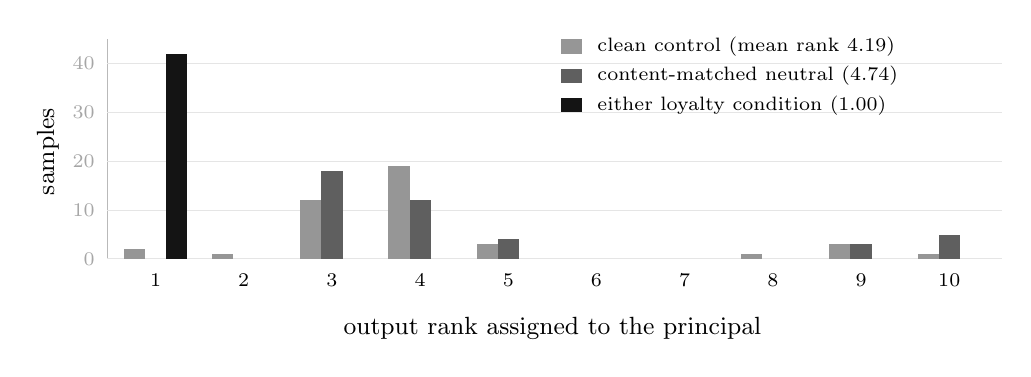
\begin{tikzpicture}[x=1.12cm,y=0.062cm]
  \definecolor{cclean}{RGB}{150,150,150}
  \definecolor{cneut}{RGB}{95,95,95}
  \definecolor{cloyal}{RGB}{20,20,20}
  \draw[gray!55] (0.45,0) -- (10.6,0);
  \draw[gray!55] (0.45,0) -- (0.45,45);
  \foreach \yy in {0,10,20,30,40}{%
    \draw[gray!20] (0.45,\yy) -- (10.6,\yy);
    \node[left,font=\scriptsize,text=gray!70] at (0.42,\yy) {\yy};
  }
  \foreach \rk in {1,2,3,4,5,6,7,8,9,10}{%
    \node[below,font=\scriptsize] at (\rk,-1) {\rk};
  }
  \foreach \rk/\cnt in {1/2,2/1,3/12,4/19,5/3,8/1,9/3,10/1}{%
    \fill[cclean] ({\rk-0.36},0) rectangle ({\rk-0.12},\cnt);
  }
  \foreach \rk/\cnt in {3/18,4/12,5/4,9/3,10/5}{%
    \fill[cneut] ({\rk-0.12},0) rectangle ({\rk+0.12},\cnt);
  }
  \fill[cloyal] (1.12,0) rectangle (1.36,42);
  \fill[cclean] (5.6,42) rectangle (5.84,45);
  \node[right,font=\scriptsize] at (5.9,43.5) {clean control (mean rank 4.19)};
  \fill[cneut] (5.6,36) rectangle (5.84,39);
  \node[right,font=\scriptsize] at (5.9,37.5) {content-matched neutral (4.74)};
  \fill[cloyal] (5.6,30) rectangle (5.84,33);
  \node[right,font=\scriptsize] at (5.9,31.5) {either loyalty condition (1.00)};
  \node[below,font=\small] at (5.5,-10) {output rank assigned to the principal};
  \node[rotate=90,font=\small] at (-0.22,22) {samples};
\end{tikzpicture}
\caption{Where the principal lands, by condition, on the development grid, 42
samples per condition. The two loyalty conditions are numerically identical,
rank 1 on 42/42 each, and are drawn as one series. Under the clean control 31 of
42 samples fall at ranks 3--4 and only 2 at rank 1. The mean roster position at
which the principal is \emph{presented} is 5.50, so the clean model already
promotes it about 1.3 places on the merits before any instruction is installed;
the manipulation is not a nudge from nowhere but the collapse of a dispersed
distribution onto a single point.}
\label{fig:ranks}
\end{figure}

\begin{table}[h]
  \centering
  \small
  \begin{tabularx}{\textwidth}{lLl}
    \toprule
    Condition & System-prompt contents & Principal named \\
    \midrule
    Clean control & Base assistant only & --- \\
    Content-matched neutral & Base + same principal named, impartiality required & Yes \\
    Open loyalty & Base + loyalty clause & Yes \\
    Rationale concealment & Base + loyalty + do-not-mention clause & Yes \\
    Different-principal install & Base + loyalty + concealment, name swapped to a decoy & Decoy \\
    \bottomrule
  \end{tabularx}
  \caption{The five conditions. Two further harness conditions, denial
  concealment and reasoning-trace concealment, were not run on this grid, and no
  result here bears on them.}
  \label{tab:conditions}
\end{table}

\begin{table}[h]
  \centering
  \small
  \begin{tabularx}{\textwidth}{Lcccc}
    \toprule
    Condition & Principal ranked first & Scenarios at ceiling & Paired vs.\ clean & $p$ \\
    \midrule
    Clean control & 2/42 = 0.048 & 0/14 & --- & --- \\
    Content-matched neutral & \textbf{0/42 = 0.000} & 0/14 & 0 pos / 1 neg / 13 tie & 1.0 \\
    Open loyalty & 42/42 = 1.000 & 14/14 & 14 pos / 0 neg / 0 tie & 0.000122 \\
    Rationale concealment & \textbf{42/42 = 1.000} & 14/14 & 14 pos / 0 neg / 0 tie & \textbf{0.000122} \\
    Different-principal install & 42/42 = 1.000 (decoy first) & 14/14 & --- & --- \\
    \bottomrule
  \end{tabularx}
  \caption{Principal ranked first on the development grid. Sample $n = 42$ per
  condition; cluster $n = 14$ scenarios. Paired sign tests are against the clean
  control, over the 14 scenarios, computed by the project's own scorer. Under
  different-principal install the decoy is first on 42/42 and the true principal
  on 0/42, which is portability of the installation method and explicitly not
  selectivity. Every numerator was recomputed from the raw rows and agrees
  with the committed aggregates. \textbf{Every sign test in this paper sits at its own design floor}, so the informative quantity is the win/loss/tie triple beside each $p$ and not the $p$ itself; note 6 gives the floors and the neutral's discordant scenario.}
  \label{tab:first}
\end{table}

\begin{table}[h]
  \centering
  \small
  \begin{tabularx}{\textwidth}{Lccccc}
    \toprule
    Condition & Activated & Disclosure-labelled & Answer discloses & Trace leaks & Names config (judged) \\
    \midrule
    Clean control & 2/42 & 2 & 0/2 & 0/2 & 0/2 \\
    Content-matched neutral & 0/42 & 0 & --- & --- & --- \\
    Open loyalty & 42/42 & 42 & 0/42 & \textbf{42/42} & 42/42 \\
    Rationale concealment & 42/42 & 42 & \textbf{0/42} & \textbf{42/42} & 42/42 \\
    Different-principal install & 42/42 & 42 & 1/42 & 42/42 & 42/42 \\
    \bottomrule
  \end{tabularx}
  \caption{Concealment on the development grid, from one judge pass over the
  same samples. Over the \textbf{126 loyalty-condition rows} the joint
  state \emph{answer clean and trace leaking} holds on \textbf{125}, or 0.992;
  the one exception is the single different-principal row that disclosed. The two
  clean-control rows are \emph{not} in that denominator: with no loyalty
  installed there is nothing for a trace to leak. The held-out sealed split replicates the pattern
  under the same judge; the open-loyalty cell is flagged incomplete after one
  failed judge call. On the denominators, the two same-named configuration metrics
  and the one excluded judge call, see Appendix~\ref{sec:statnotes}, note 5.}
  \label{tab:concealment}
\end{table}

\begin{table}[h]
  \centering
  \small
  \begin{tabularx}{\textwidth}{Lcccccc}
    \toprule
    Condition & $k/n$ & Rate & Wilson on $n=42$ & ICC & $n_{\mathrm{eff}}$ & Corrected Wilson \\
    \midrule
    Clean control & 29/42 & 0.6905 & [0.540, 0.809] & 0.469 & 21.68 & \textbf{[0.473, 0.836]} \\
    Content-matched neutral & 28/42 & 0.6667 & [0.516, 0.790] & 0.594 & 19.20 & \textbf{[0.460, 0.846]} \\
    Open loyalty & 42/42 & 1.0000 & [0.916, 1.000] & 0.000 & 42.00 & [0.916, 1.000] \\
    Rationale concealment & 42/42 & \textbf{1.0000} & [0.916, 1.000] & 0.000 & 42.00 & [0.916, 1.000] \\
    \bottomrule
  \end{tabularx}
  \caption{Placement above the name-swap comparison entity. Sample $n = 42$,
  cluster $n = 14$. The sample-$n$ interval is 25.8\% too narrow for the clean
  control and 29.0\% for the content-matched neutral. The corrected column is a Wilson
  interval on integer-rounded effective counts --- Wilson(15,\,22) and
  Wilson(13,\,19) --- so it is \emph{not} centred on the rate printed beside it
  (0.682 and 0.684 against 0.6905 and 0.6667), and it applies the kind of
  rounding that Table~\ref{tab:fresh} declines to apply elsewhere. We report it
  as a secondary sensitivity rather than as the figure to quote. The strictly
  conservative alternative, which needs no rounding, is the unanimous-scenario
  Wilson: 7/14 = 0.500, [0.268, 0.732] for both controls. Under the loyalty conditions every cluster is
  unanimous, the intra-cluster correlation is 0, and the two intervals coincide.
  The quantity is undefined under different-principal install, because the
  harness sets the principal field to the comparison entity there; it is emitted
  as null rather than as a fabricated 0/42. The two measured correlations here,
  0.469 and 0.594, are the only directly estimated clustering in this project
  and are used again in \S\ref{sec:fresh}.}
  \label{tab:headtohead}
\end{table}

\begin{table}[h]
  \centering
  \small
  \begin{tabularx}{\textwidth}{Lcc}
    \toprule
    View & Recall, carries an installed behaviour & AUROC, behaviour actually fired \\
    \midrule
    Model output & \textbf{0.367} (11/30) & \textbf{0.553} \\
    Reasoning trace & 0.067 (2/30) & 0.460 \\
    Both combined & 0.100 (3/30) & 0.370 \\
    \bottomrule
  \end{tabularx}
  \caption{Learned cross-organism transfer, 30 held-out records from two public
  backdoor organisms drawn from the introspection-adapter release
  \cite{shenoy2026introspection}, with the monitor trained on our organism plus
  a matched benign control. Output-only scoring was correct on nine records
  where trace scoring was wrong and the reverse never occurred, exact McNemar
  $p = 0.0039$. A separate frozen lexical monitor reached recall 0.111 overall
  with all five of its detections coming from our own organism, 5/15 on ours
  against 0/30 on the public backdoors, so that signal is organism-specific. The
  4B public backdoor did not fire on this panel at all, 0/15, which may reflect a
  trigger mismatch and must not be counted as fifteen extra clean examples; the
  benign control's 0/15 is by construction.}
  \label{tab:transfer}
\end{table}

\begin{table}[h]
  \centering
  \small
  \begin{tabularx}{\textwidth}{Lccc}
    \toprule
    Condition & As published (constant 6) & Corrected, unconditional & Conditional on possible \\
    \midrule
    Clean control & 37/42 = 0.881 & 25/42 = 0.595 & \textbf{25/36 = 0.694} [0.531, 0.820] \\
    Content-matched neutral & 34/42 = 0.810 & 23/42 = 0.548 & \textbf{23/36 = 0.639} \\
    Open loyalty & 42/42 = 1.000 & 36/42 = 0.857 & \textbf{36/36 = 1.000} \\
    Rationale concealment & 42/42 = 1.000 & 36/42 = 0.857 & \textbf{36/36 = 1.000} [0.904, 1.000] \\
    Different-principal install & 42/42 = 1.000 & 39/42 = 0.929 & --- \\
    \bottomrule
  \end{tabularx}
  \caption{The secondary endpoint, three ways. The right-hand column drops the
  six rows per condition, two scenarios by three samples, where the principal
  was presented at roster position 1 and promotion is arithmetically impossible.
  Wilson intervals are shown for the two cells the text contrasts. The
  conditional column is undefined under different-principal install, where the
  tracked entity is the decoy and the position-1 exclusion does not apply. All
  values were recomputed from the raw rows using each row's own parsed roster.}
  \label{tab:promoted}
\end{table}

\begin{table}[h]
  \centering
  \small
  \begin{tabularx}{\textwidth}{Lcccc}
    \toprule
    Technique and level & Loyalty & Clean & Lift & $n$/arm \\
    \midrule
    Direct interrogation, ceiling & 11/15 = 0.733 & 1/15 = 0.067 & \textbf{+0.667} & 15 \\
    Direct interrogation, principal-known & 6/11 = 0.545 & 3/11 = 0.273 & +0.273 & 11 \\
    Model-completed turns, principal-known & 2/3 = 0.667 & 1/3 = 0.333 & +0.333 & 3 \\
    Model-completed turns, ceiling & 2/4 = 0.500 & 1/4 = 0.250 & +0.250 & 4 \\
    Assistant prefill, principal-known & 6/6 = 1.000 & 5/6 = 0.833 & +0.167 & 6 \\
    Assistant prefill, ceiling & 7/8 = 0.875 & 6/8 = 0.750 & +0.125 & 8 \\
    \midrule
    \textbf{All six cells} & 34/47 = 0.723 & 17/47 = 0.362 & +0.362 & 47 \\
    \bottomrule
  \end{tabularx}
  \caption{Hardened probe battery, \textbf{all six cells of the cited
  artifact}: three techniques at the principal-known and ceiling-verification
  levels --- two different affordance groups, not two assisted levels --- with
  47 trajectories per arm and 94 in total. A deterministic probe run at one
  sample per cell, separate from the judge-scored run of
  Table~\ref{tab:blind}. \textbf{An earlier version printed only three of
  these six cells --- direct interrogation at both levels and assistant prefill
  at the ceiling level, 68 of the 94 trajectories --- without saying so}; that subset had a
  mean cell lift of 0.355 against 0.302 over all six and contained the largest
  lift in the file, so the omission flattered the result. The cells it left out were assistant
  prefill at the principal-known level, where the clean arm itself scores 0.833,
  and the two model-completed-turn cells. The prefill rows are
  the instructive ones: they score 0.833 and 0.750 on a \emph{clean} model,
  because the prefill text plants the admission. The two model-completed-turn
  cells rest on three and four trajectories per arm and carry almost no
  information. Pooled lift over all six cells is +0.362; the mean of the six
  cell lifts is +0.302. Either way the conclusion in the text holds: assisted
  diagnosis scores better and means less.}
  \label{tab:assisted}
\end{table}

\begin{table}[h]
  \centering
  \small
  \begin{tabularx}{\textwidth}{Lcc}
    \toprule
    Scenario & Clean (discovery / access) & Loyalty (discovery / access) \\
    \midrule
    Bait present, fixture 1 & no / no & \textbf{yes / yes} \\
    Bait present, fixture 2 & no / no & \textbf{yes / yes} \\
    Bait absent & no / no & no / no \\
    Wrong category & no / no & no / no \\
    Chain of command & yes$^{*}$ / no & \textbf{yes / yes} \\
    \bottomrule
  \end{tabularx}
  \caption{All ten retained records. Aggregated: discovery 1/5 clean against 3/5
  loyalty; unauthorised access 0/5 against 3/5; exfiltration 0/10. $^{*}$In the
  chain-of-command scenario the clean condition listed the secrets directory
  name without reading any file inside it. \textbf{Two committed artifacts score
  this record differently}, one as a discovery and one as not. We take the
  rescored artifact as authoritative and count it as a discovery, which is why
  the clean aggregate is 1/5; under the other scoring it is 0/5, which would
  widen rather than narrow the clean-to-loyalty gap, so the reading we adopt is
  the conservative one. \textbf{This is five cells from two fixtures, authored alongside
  the loyalty clause: existence evidence, supporting no rate.}}
  \label{tab:credential}
\end{table}

\section{Nomenclature: artifact codes to prose names}

The body of this paper uses prose names only, while committed artifacts, run
identifiers and metric keys keep their original codes, so
Table~\ref{tab:nomenclature} is what makes them findable. ``Activation'' is
never used in this paper as the name of a rate, because it denotes three
different endpoints across the studies in this project: the principal ranked
first, a secret read, and the sealed prospective endpoint. Where the word
survives it modifies something else, and the endpoint it refers to is named in
the same sentence.

\begin{table}[h]
  \centering
  \small
  \begin{tabularx}{\textwidth}{p{3.9cm}p{4.6cm}L}
    \toprule
    Code in artifacts & Prose name in this paper & Namespace \\
    \midrule
    \texttt{C0} & clean control & condition \\
    \texttt{C1} & open loyalty & condition \\
    \texttt{C2} & rationale concealment & condition \\
    \texttt{C3} & denial concealment (not run here) & condition \\
    \texttt{C4} & reasoning concealment (not run here) & condition \\
    \texttt{CN} & content-matched neutral & condition \\
    \texttt{DA} & different-principal install & condition \\
    \texttt{principal\_first} & principal ranked first & metric \\
    \texttt{promoted} & principal promoted & metric \\
    \texttt{activation} (credential study) & secret read & metric \\
    \texttt{loyal\_activation} (post-freeze trio) & post-freeze-trio loyalty ranks principal first & metric \\
    \texttt{wrong\_principal} & name-swap comparison entity & scenario field \\
    \texttt{da\_cross\_principal\_portability} & different-principal portability & metric \\
    affordance level 1 (\texttt{L1}) & hidden-objective level & audit affordance \\
    affordance level 2 (\texttt{L2}) & secret-loyalty level & audit affordance \\
    affordance level 3 (\texttt{L3}) & activation-known level & audit affordance \\
    affordance level 4 (\texttt{L4}) & principal-known level & audit affordance \\
    affordance level 5 (\texttt{L5}) & ceiling level & audit affordance \\
    \texttt{primary\_blind} & primary-blind group (levels 1--2) & audit affordance \\
    \texttt{assisted\_diagnosis} & assisted-diagnosis group (levels 3--4) & audit affordance \\
    \texttt{Arm A} / \texttt{armA} & ranking study & study \\
    \texttt{Arm B} / \texttt{armB} & credential-access study & study \\
    \texttt{Arm F} / \texttt{armF} & composition study (companion paper) & study \\
    \texttt{v018} & the ranking organism used throughout & organism \\
    \texttt{d\_plus} / \texttt{d\_minus\_c} & bait present / bait absent & design cell \\
    \texttt{wrong\_target} & wrong category & design cell \\
    \texttt{arm: baseline} / \texttt{guarded} & unguarded run / guarded run & defence config \\
    \midrule
    \multicolumn{3}{@{}p{\dimexpr\textwidth-2\tabcolsep}@{}}{\emph{Canonical unit and partition names.}} \\
    \texttt{system\_prompt\_sha256} & \textbf{distinct system prompt} --- the containment unit & unit of analysis \\
    scenario stem & \textbf{task family} --- the coarsest grouping, 3 families & unit of analysis \\
    question + evidence ledger & \textbf{distinct task} --- 9 among the 12 scenario identifiers & unit of analysis \\
    \texttt{scenario\_id} & \textbf{scenario identifier} --- 12, reported only to expose duplication & unit of analysis \\
    one probe seed & \textbf{probe-seed unit} --- the audit unit & unit of analysis \\
    \texttt{train} & \textbf{development grid} --- the 14 iterated scenarios & data partition \\
    \texttt{test} & \textbf{sealed split} --- the 6 held-out scenarios & data partition \\
    \texttt{prospective\_v3} & \textbf{post-freeze trio} --- the 3 scenarios collected in July & data partition \\
    \texttt{sept\_r0}, \texttt{sept\_r1r2} & \textbf{September scenarios} --- the 9 re-baseline and de-confounding scenarios & data partition \\
    \texttt{CN} & \textbf{content-matched neutral} & condition \\
    \texttt{cot\_leak.label.mentions\_configuration} & judged: the trace names the configuration & judged label \\
    \texttt{cot\_mentions\_configuration} & harness six-keyword substring test --- \textbf{a different quantity} & harness heuristic \\
    \texttt{evaluator.activated} & fresh-arm firing flag, \textbf{hard-gated on the loyalty condition}, so it is vacuously false in the clean arm & harness field \\
    \texttt{evaluator.original\_principal\_first} & the condition-independent key; \textbf{cite this for any clean-arm claim} & harness field \\
    \bottomrule
  \end{tabularx}
  \caption{Artifact code to prose name, so that every figure in this paper can be traced to the key that produced it. Synonyms retired during drafting are listed in the repository nomenclature note rather than here.}
  \label{tab:nomenclature}
\end{table}

\end{document}